\documentclass[11pt]{article}

% --- Encoding and language -------------------------------------------------
\usepackage[T1]{fontenc}
\usepackage[utf8]{inputenc}
\usepackage[english]{babel} % switch to [polish] + translate headings if required

% --- Layout ----------------------------------------------------------------
\usepackage[a4paper,margin=2.5cm]{geometry}
\usepackage{parskip}
\raggedbottom

% --- Math, units, chemistry ------------------------------------------------
\usepackage{amsmath}
\usepackage{siunitx}
\usepackage[version=4]{mhchem}

% --- Figures and tables ----------------------------------------------------
\usepackage{graphicx}
\usepackage{subcaption}
\usepackage{booktabs}
\usepackage{placeins}
\graphicspath{{assets/}{../results/figures/}{../results/diagnostics/}}

% --- References ------------------------------------------------------------
\usepackage[numbers,sort&compress]{natbib}
\usepackage{hyperref}
\renewcommand{\refname}{Bibliography}

\sisetup{detect-all}
\DeclareSIUnit{\atmosphere}{atm}

\title{Numerical Study of Hydrogen-Enriched Methane--Air Combustion\\
       Using Detailed Chemical Kinetics}
\author{Jan Burghardt\\
        \small Faculty of Power and Aeronautical Engineering,
        Warsaw University of Technology\\
        \small Computer Methods in Combustion (MKWS)}
\date{June 16, 2026}

\begin{document}
\pagenumbering{gobble}
\begin{titlepage}
  \centering
  \vspace*{1.0cm}
  
\includegraphics[width=0.40\textwidth]{meil_pw_logo.png}\par
  \vspace{1.0cm}
  {\Large Politechnika Warszawska\par}
  \vspace{0.25cm}
  {\large Wydział Mechaniczny Energetyki i Lotnictwa\par}
  \vspace{1.2cm}
  {\large Metody komputerowe w spalaniu\par}
  \vfill
  {\LARGE\bfseries Numerical Study of Hydrogen-Enriched Methane--Air Combustion\par}
  \vspace{0.35cm}
  {\Large Using Detailed Chemical Kinetics\par}
  \vfill
  {\large Author: Jan Burghardt\par}
  \vspace{0.25cm}
  {\large Date: June 16, 2026\par}
  \vspace*{1.0cm}
\end{titlepage}
\clearpage
\pagenumbering{arabic}

\begin{abstract}
This work investigates the effect of hydrogen enrichment on the combustion of
methane--air mixtures using detailed chemical kinetics in Cantera with the
GRI-Mech~3.0 mechanism. Hydrogen fraction in the fuel was varied from
\SI{0}{\percent} to \SI{40}{\percent} (molar) across a range of equivalence
ratios. Adiabatic equilibrium states, autoignition delay times, laminar flame
speeds, and a perfectly stirred combustor were analysed. At $\phi=1.0$,
\SI{300}{\kelvin} and \SI{1}{\atmosphere}, the calculated laminar flame speed
increased from \SI{37.68}{\centi\meter\per\second} for methane--air to
\SI{52.16}{\centi\meter\per\second} for \SI{40}{\percent}
hydrogen in the fuel. At $T_0=\SI{1000}{\kelvin}$,
$p=\SI{10}{\atmosphere}$ and $\phi=1.0$, the constant-pressure ignition delay
decreased from \SI{81.99}{\milli\second} to
\SI{12.64}{\milli\second} over the same enrichment range. The perfectly
stirred reactor results identify stability-transition brackets between cold
extinguished and hot stable steady-state solutions on the tested
residence-time grid.
\end{abstract}

\clearpage
\tableofcontents
\clearpage

\section*{Nomenclature}
\addcontentsline{toc}{section}{Nomenclature}
\begin{center}
  \begin{tabular}{ll}
    \toprule
    Symbol & Meaning \\
    \midrule
    $\phi$ & equivalence ratio \\
    $\tau_\mathrm{ign}$ & ignition delay \\
    $\tau_\mathrm{res}$ & residence time \\
    $S_L$ & laminar flame speed \\
    $T_\mathrm{ad}$ & adiabatic flame temperature \\
    $X_i$ & mole fraction of species $i$ \\
    $Y_i$ & mass fraction of species $i$ \\
    $p$ & pressure \\
    $T_0$ & initial temperature \\
    $\dot{m}$ & mass-flow rate \\
    \bottomrule
  \end{tabular}
\end{center}

\clearpage

% ===========================================================================
\section{Introduction}
Hydrogen is widely studied as a clean fuel for gas-fired combustors and
turbines, and blending hydrogen into methane is a practical near-term route to
lowering carbon emissions from existing equipment \citep{bdaiwi2024}.
Published experimental and review studies report that hydrogen enrichment
generally increases laminar burning velocity and changes ignition and flame
stability characteristics. Its implications for flashback and nitrogen-oxide
formation depend strongly on mixture composition and operating conditions
\citep{li2017,bdaiwi2024}.

In an engineering context, hydrogen can be added to existing gaseous fuels as
part of fuel-flexibility or decarbonisation studies for gas-turbine or
aero-engine combustor concepts. Such changes affect ignition propensity,
laminar flame speed, flame temperature and combustion stability. The models
used here are therefore treated as preliminary trend-analysis tools for
\ce{CH4}/\ce{H2}--air mixtures, not as a complete combustor model.

The objective of this study is to quantify, with a single consistent kinetic
model, how the molar hydrogen fraction in a \ce{CH4}/\ce{H2} fuel blend affects:
(i) the adiabatic flame temperature and equilibrium product composition;
(ii) the autoignition delay time and its sensitivity to temperature, pressure
and equivalence ratio; (iii) the laminar flame speed; and (iv) the behaviour
of an ideal perfectly stirred combustor on a prescribed residence-time grid.

\clearpage

% ===========================================================================
\section{Methodology}

\subsection{Project workflow}
The calculations are organised around a common definition of fuel composition,
oxidizer composition and operating-condition grids. Table~\ref{tab:workflow} summarises the computational workflow; it is a
project organisation diagram rather than a statement that all models are
physically coupled in sequence.

\begin{table}[htbp]
  \centering
  \caption{Computational workflow used in the project.}
  \label{tab:workflow}
  \begin{tabular}{c}
    \toprule
    Configuration and fuel definition \\
    $\downarrow$ \\
    Equilibrium analysis \\
    $\downarrow$ \\
    Ignition-delay analyses \\
    $\downarrow$ \\
    PSR residence-time analysis \\
    $\downarrow$ \\
    FreeFlame analysis \\
    $\downarrow$ \\
    CSV outputs and figures \\
    $\downarrow$ \\
    Report \\
    \bottomrule
  \end{tabular}
\end{table}

\subsection{Chemical mechanism}
All simulations were performed with Cantera \citep{cantera} using the
GRI-Mech~3.0 mechanism \citep{grimech30}, an optimised detailed mechanism for
natural-gas combustion comprising 53~species and 325~reactions and including
nitrogen chemistry for \ce{NO} formation. The mechanism is well suited to
methane-dominated mixtures; its applicability to high hydrogen fractions is
discussed in Section~\ref{sec:limitations}.

\subsection{Fuel mixture definition}
The fuel is a binary \ce{CH4}/\ce{H2} blend parameterised by the molar hydrogen
fraction
\begin{equation}
  x_{\ce{H2}} = \frac{n_{\ce{H2}}}{n_{\ce{H2}} + n_{\ce{CH4}}},
\end{equation}
so that the fuel composition is $\{\ce{CH4}: 1-x_{\ce{H2}},\ \ce{H2}: x_{\ce{H2}}\}$.
Air is modelled as \ce{O2} $+ 3.76\,\ce{N2}$, and the mixture is set with a
prescribed equivalence ratio~$\phi$.

\subsection{Adiabatic equilibrium}
Equilibrium states are obtained at constant enthalpy and pressure
($\mathrm{HP}$ problem), giving the adiabatic flame temperature and the
equilibrium mole fractions of \ce{NO}, \ce{CO}, \ce{CO2} and \ce{H2O}. The
initial state is $T_0=\SI{900}{\kelvin}$ and
$p=\SI{10}{\atmosphere}$. The tested equivalence-ratio grid is
$\phi=0.6$, 0.8, 1.0, 1.2 and 1.4, and the hydrogen fractions in the fuel
blend are 0, 10, 20, 30 and \SI{40}{\mole\percent}.

\subsection{Autoignition delay}
Autoignition is computed in a homogeneous adiabatic reactor, modelled both as a
constant-volume (\texttt{IdealGasReactor}) and a constant-pressure
(\texttt{IdealGasConstPressureReactor}) system. The ignition delay~$\tau$ is
defined as the time of maximum temperature-rise rate, $\max(\mathrm{d}T/\mathrm{d}t)$;
the time of peak \ce{OH} mass fraction is used as an independent cross-check.
The primary temperature sweep uses the constant-pressure reactor at
$\phi=1.0$, $p=\SI{10}{\atmosphere}$, $T_0=900$, 950, 1000, 1050 and
\SI{1100}{\kelvin}, with hydrogen fractions of 0, 10, 20, 30 and
\SI{40}{\mole\percent}. The pressure sweep uses $T_0=\SI{1000}{\kelvin}$,
$\phi=1.0$, pressures of 5, 10 and \SI{20}{\atmosphere}, and hydrogen
fractions of 0, 20 and \SI{40}{\mole\percent}. The equivalence-ratio sweep
uses $T_0=\SI{1000}{\kelvin}$, $p=\SI{10}{\atmosphere}$, $\phi=0.6$ to 1.4
in increments of 0.1, and hydrogen fractions of 0, 20 and
\SI{40}{\mole\percent}.

\subsection{Laminar flame speed}
The laminar flame speed is obtained from a one-dimensional freely propagating
premixed flame (\texttt{FreeFlame}) with adaptive grid refinement. The final
calculations use multicomponent transport with Soret diffusion enabled. The
reported speed is the unburned-gas inlet velocity of the converged solution.
Reference conditions are an unburned temperature of \SI{300}{\kelvin} and a
pressure of \SI{1}{\atmosphere}, chosen so that the stoichiometric methane--air
result can be used as a reference consistency check
(Section~\ref{sec:flamespeed}). The domain width is \SI{0.03}{\meter}; the
tested equivalence ratios are $\phi=0.6$, 0.8, 1.0, 1.2 and 1.4; and the
hydrogen fractions are 0, 20 and \SI{40}{\mole\percent}. Grid refinement uses
ratio = 3.0, slope = 0.06 and curve = 0.12.

\subsection{Perfectly stirred reactor}
A perfectly stirred reactor (PSR) is built from an inlet reservoir, an
\texttt{IdealGasReactor} and an exhaust reservoir, coupled by a
\texttt{MassFlowController} and a \texttt{PressureController}. The inlet mass
flow is set as $\dot{m} = \frac{m_\mathrm{reactor}}{\tau_\mathrm{res}}$, allowing the
residence time~$\tau_\mathrm{res}$ to be swept. The PSR is zero-dimensional,
adiabatic and perfectly stirred. It is initialised from equilibrium products at
the inlet enthalpy and pressure, then continued from long to short residence
time; as a result, the calculated sequence follows the hot burning branch
where that branch is available. The steady state is solved at each tested
residence time to identify a stability-transition bracket between cold
extinguished and hot stable steady-state solutions on the discrete grid. The
inlet temperature is \SI{1000}{\kelvin}, the pressure is
\SI{10}{\atmosphere}, the tested equivalence ratios are $\phi=0.7$ and 1.0,
and the hydrogen fractions are 0, 20 and \SI{40}{\mole\percent}. The
residence-time grid is 0.001 to \SI{50}{\milli\second} as configured, and the
hot-gas residence time is $\tau=\frac{m_\mathrm{ss}}{\dot{m}}$. Equilibrium-product
initialisation is used before continuation. A \SI{500}{\kelvin} temperature
rise is used as the operational classification threshold between extinguished
and stable cases.

\subsection{Summary of analysis scope}
Table~\ref{tab:analysis-scope} collects the operating ranges used in the
individual calculations. The entries are taken from the project configuration
and the generated CSV files; they also indicate which result from each model
is used in the discussion.

\begin{table}[htbp]
  \centering
  \caption{Scope of the numerical analyses.}
  \label{tab:analysis-scope}
  \small
  \resizebox{\textwidth}{!}{%
  \begin{tabular}{lllllll}
    \toprule
    Analysis & Model & Temperature & Pressure & $\phi$ & \ce{H2} & Main result \\
    \midrule
    Equilibrium & HP equilibrium & \SI{900}{\kelvin} &
    \SI{10}{\atmosphere} & 0.6--1.4 & 0--40\% &
    $T_\mathrm{ad}$, \ce{NO}, \ce{CO} \\
    Ignition & CP reactor & 900--\SI{1100}{\kelvin} &
    \SI{10}{\atmosphere} & 1.0 & 0--40\% &
    ignition delay \\
    CV/CP comparison & homogeneous reactors & 900, 1000, \SI{1100}{\kelvin} &
    \SI{10}{\atmosphere} & 1.0 & 0, 20, 40\% &
    CP--CV delay change \\
    Pressure sweep & CP reactor & \SI{1000}{\kelvin} &
    5, 10, \SI{20}{\atmosphere} & 1.0 & 0, 20, 40\% &
    pressure sensitivity \\
    $\phi$ sweep & CP reactor & \SI{1000}{\kelvin} &
    \SI{10}{\atmosphere} & 0.6--1.4 & 0, 20, 40\% &
    delay and $T_\mathrm{max}$ \\
    PSR & ideal stirred reactor & \SI{1000}{\kelvin} &
    \SI{10}{\atmosphere} & 0.7, 1.0 & 0, 20, 40\% &
    stability-transition bracket \\
    FreeFlame & 1-D premixed flame & \SI{300}{\kelvin} &
    \SI{1}{\atmosphere} & 0.6--1.4 & 0, 20, 40\% &
    laminar flame speed \\
    \bottomrule
  \end{tabular}%
  }
\end{table}

\clearpage

% ===========================================================================
\section{Results and discussion}

\subsection{Key numerical results}
The main project-level results are summarised in
Table~\ref{tab:key-results}. The PSR entry is intentionally reported only as a
stability-transition bracket on the tested residence-time grid.

\begin{table}[htbp]
  \centering
  \caption{Selected headline results for methane--air and the
           \SI{40}{\percent} hydrogen fuel blend.}
  \label{tab:key-results}
  \resizebox{\textwidth}{!}{%
  \begin{tabular}{llll}
    \toprule
    Quantity & Conditions & 0\% \ce{H2} & 40\% \ce{H2} \\
    \midrule
    Laminar flame speed &
    $\phi=1.0$, \SI{300}{\kelvin}, \SI{1}{\atmosphere} &
    \SI{37.68}{\centi\meter\per\second} &
    \SI{52.16}{\centi\meter\per\second} \\
    Ignition delay &
    $\phi=1.0$, \SI{1000}{\kelvin}, \SI{10}{\atmosphere} &
    \SI{81.99}{\milli\second} &
    \SI{12.64}{\milli\second} \\
    Stoichiometric $T_\mathrm{ad}$ &
    HP equilibrium, \SI{900}{\kelvin}, \SI{10}{\atmosphere} &
    \SI{2595.74}{\kelvin} &
    \SI{2622.25}{\kelvin} \\
    PSR stability-transition bracket &
    $\phi=1.0$, \SI{1000}{\kelvin}, \SI{10}{\atmosphere} &
    0.002--\SI{0.005}{\milli\second} &
    0.002--\SI{0.005}{\milli\second} \\
    \bottomrule
  \end{tabular}%
  }
\end{table}

\subsection{Adiabatic flame temperature and equilibrium composition}
On the tested five-point equivalence-ratio grid, the maximum adiabatic flame
temperature is observed at $\phi=1.0$ for every fuel blend
(Figure~\ref{fig:tad}). For methane--air, $T_\mathrm{ad}$ increases from
\SI{2134.18}{\kelvin} at $\phi=0.6$ to \SI{2595.74}{\kelvin} at $\phi=1.0$,
then decreases to \SI{2427.90}{\kelvin} at $\phi=1.4$. With
\SI{40}{\mole\percent} hydrogen in the fuel, the corresponding values are
\SI{2161.47}{\kelvin}, \SI{2622.25}{\kelvin} and
\SI{2480.57}{\kelvin}. Hydrogen enrichment therefore raises the
stoichiometric equilibrium temperature by \SI{26.51}{\kelvin} over the tested
range.

The equilibrium \ce{NO} mole fraction is largest near the lean side of the
tested range: for methane--air it is 0.007842 at $\phi=0.8$, 0.004817 at
$\phi=1.0$ and 0.000163 at $\phi=1.4$. At
\SI{40}{\mole\percent} hydrogen, the corresponding values are 0.008123,
0.004987 and 0.000224. Equilibrium \ce{CO} is very small on the lean side and
increases strongly for rich mixtures, from 0.000256 at $\phi=0.6$ to 0.078503
at $\phi=1.4$ for methane--air, and from 0.000266 to 0.067442 for the
\SI{40}{\mole\percent} hydrogen blend. These equilibrium mole fractions must
not be interpreted as actual engine emissions: they represent infinite-time
adiabatic chemical equilibrium at fixed enthalpy and pressure, without finite
residence time, turbulent mixing, heat loss, or exhaust quenching.

\begin{figure}[tbp]
  \centering
  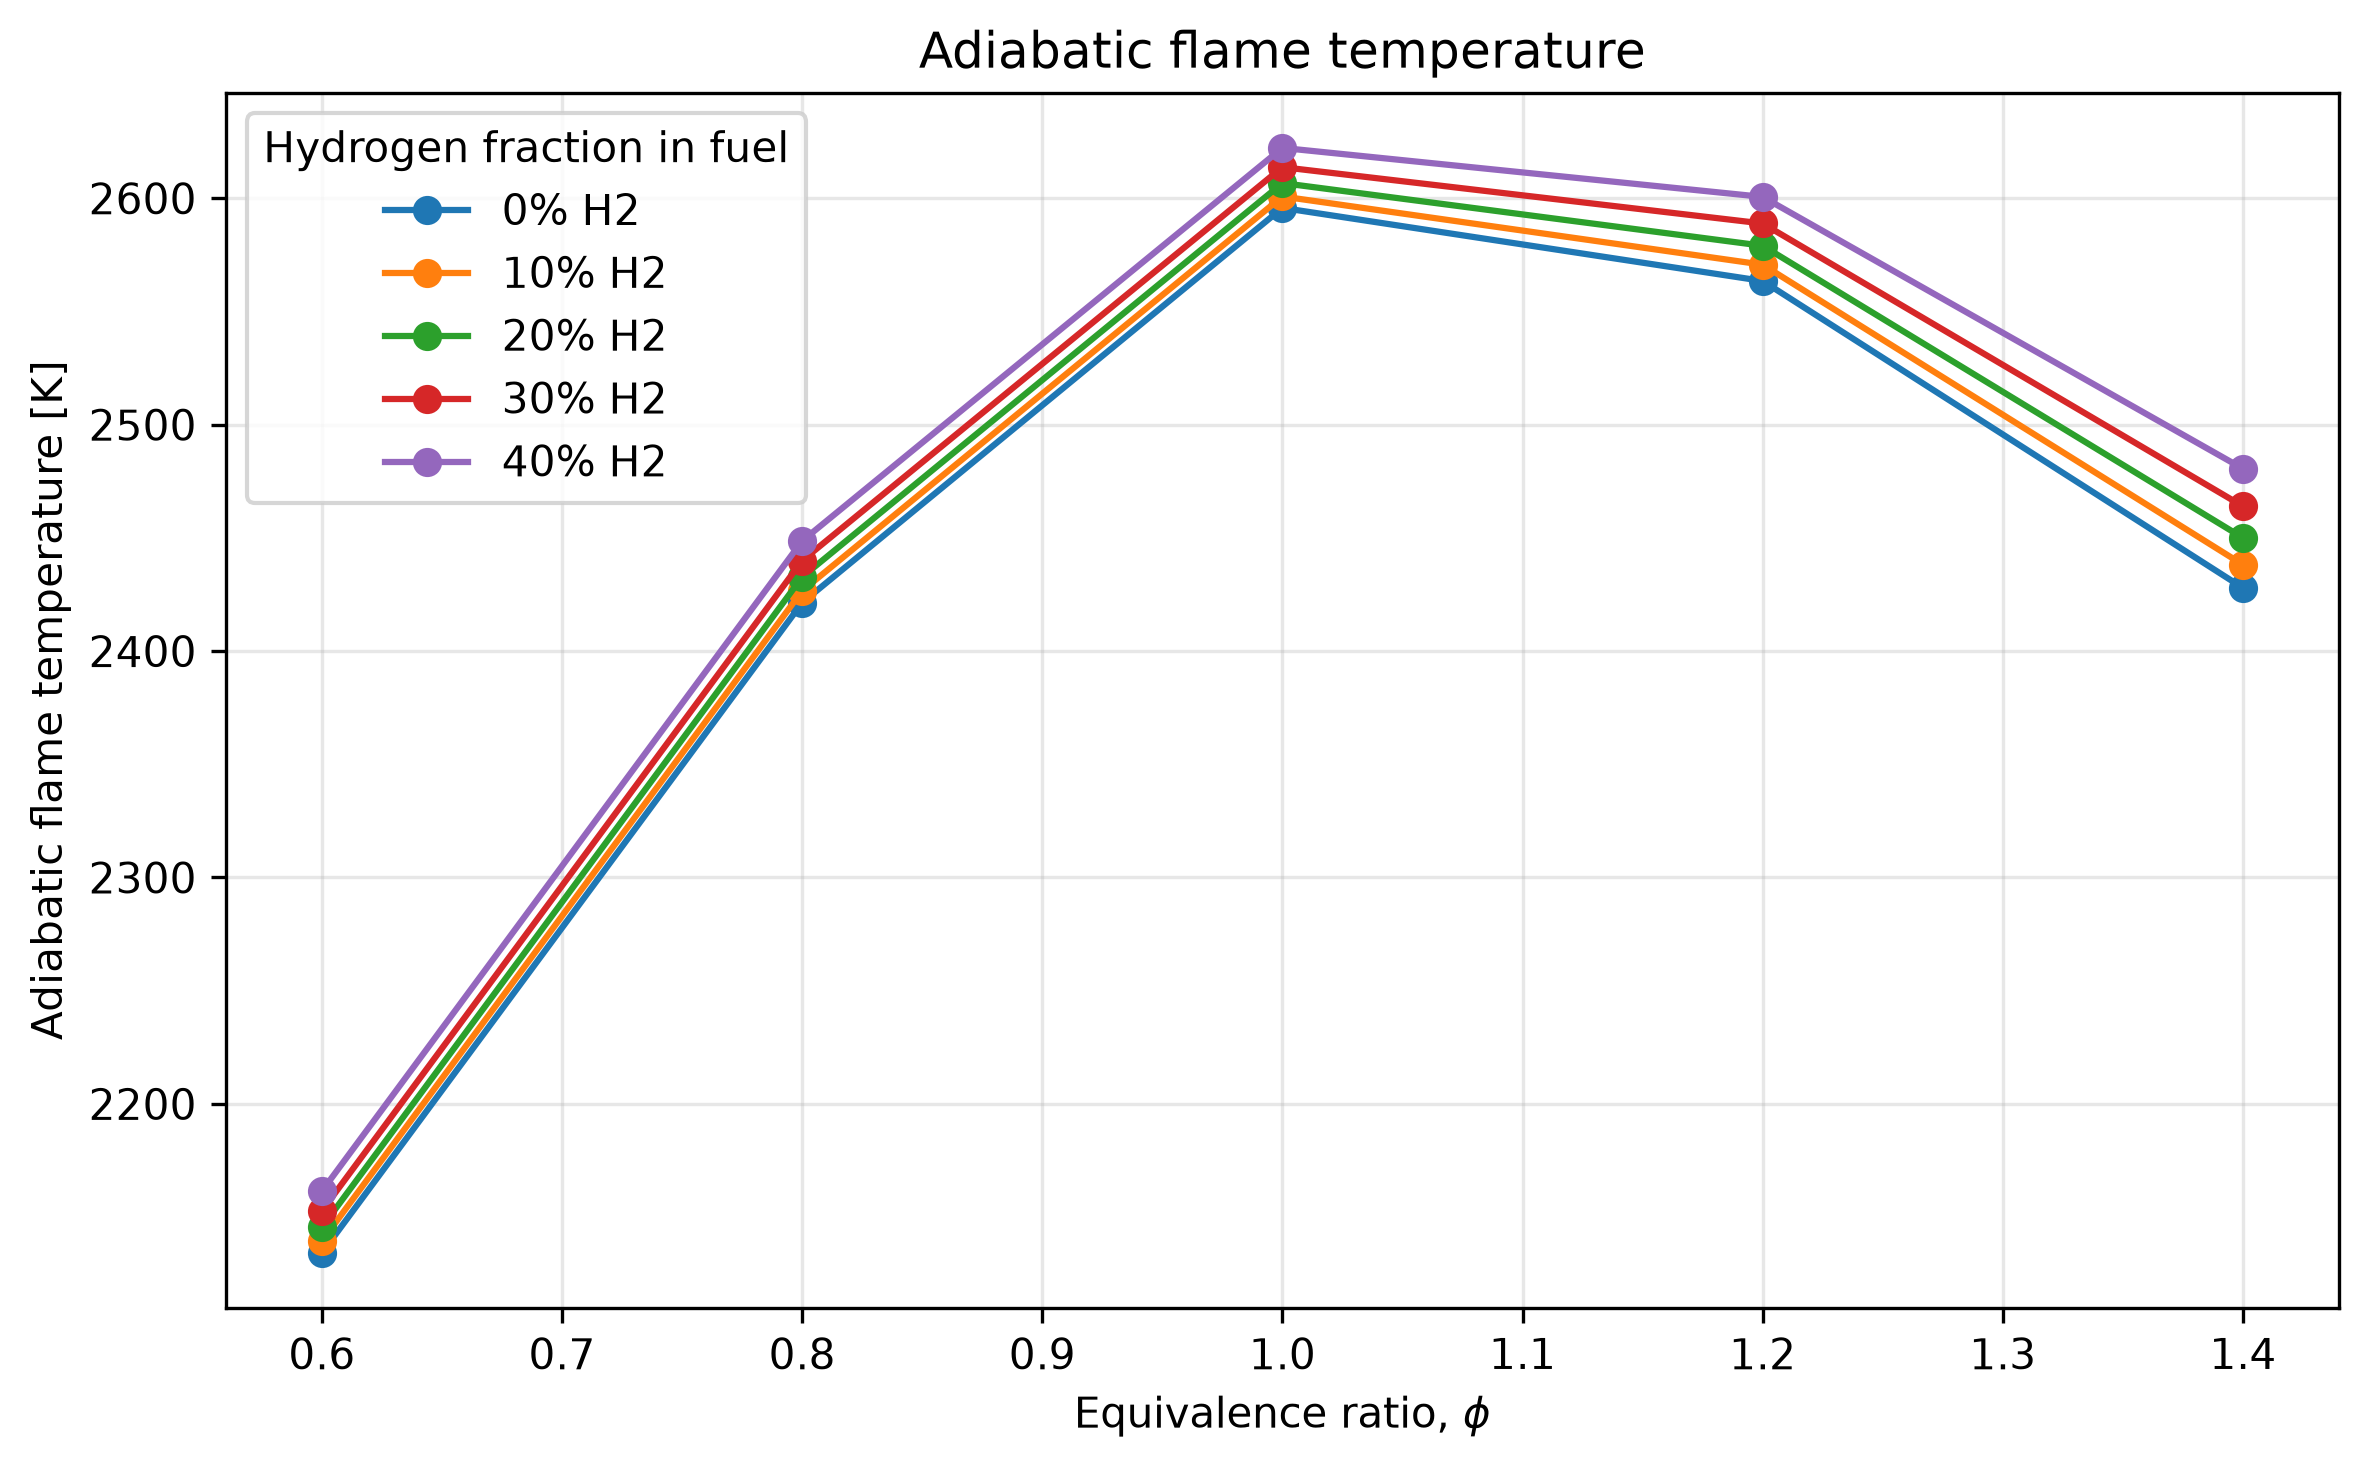
\includegraphics[width=0.78\textwidth]{tad_vs_phi.png}
  \caption{Adiabatic flame temperature versus equivalence ratio for
           different hydrogen fractions at $T_0=\SI{900}{\kelvin}$ and
           $p=\SI{10}{\atmosphere}$.}
  \label{fig:tad}
\end{figure}

\begin{figure}[tbp]
  \centering
  \begin{subfigure}{0.49\textwidth}
    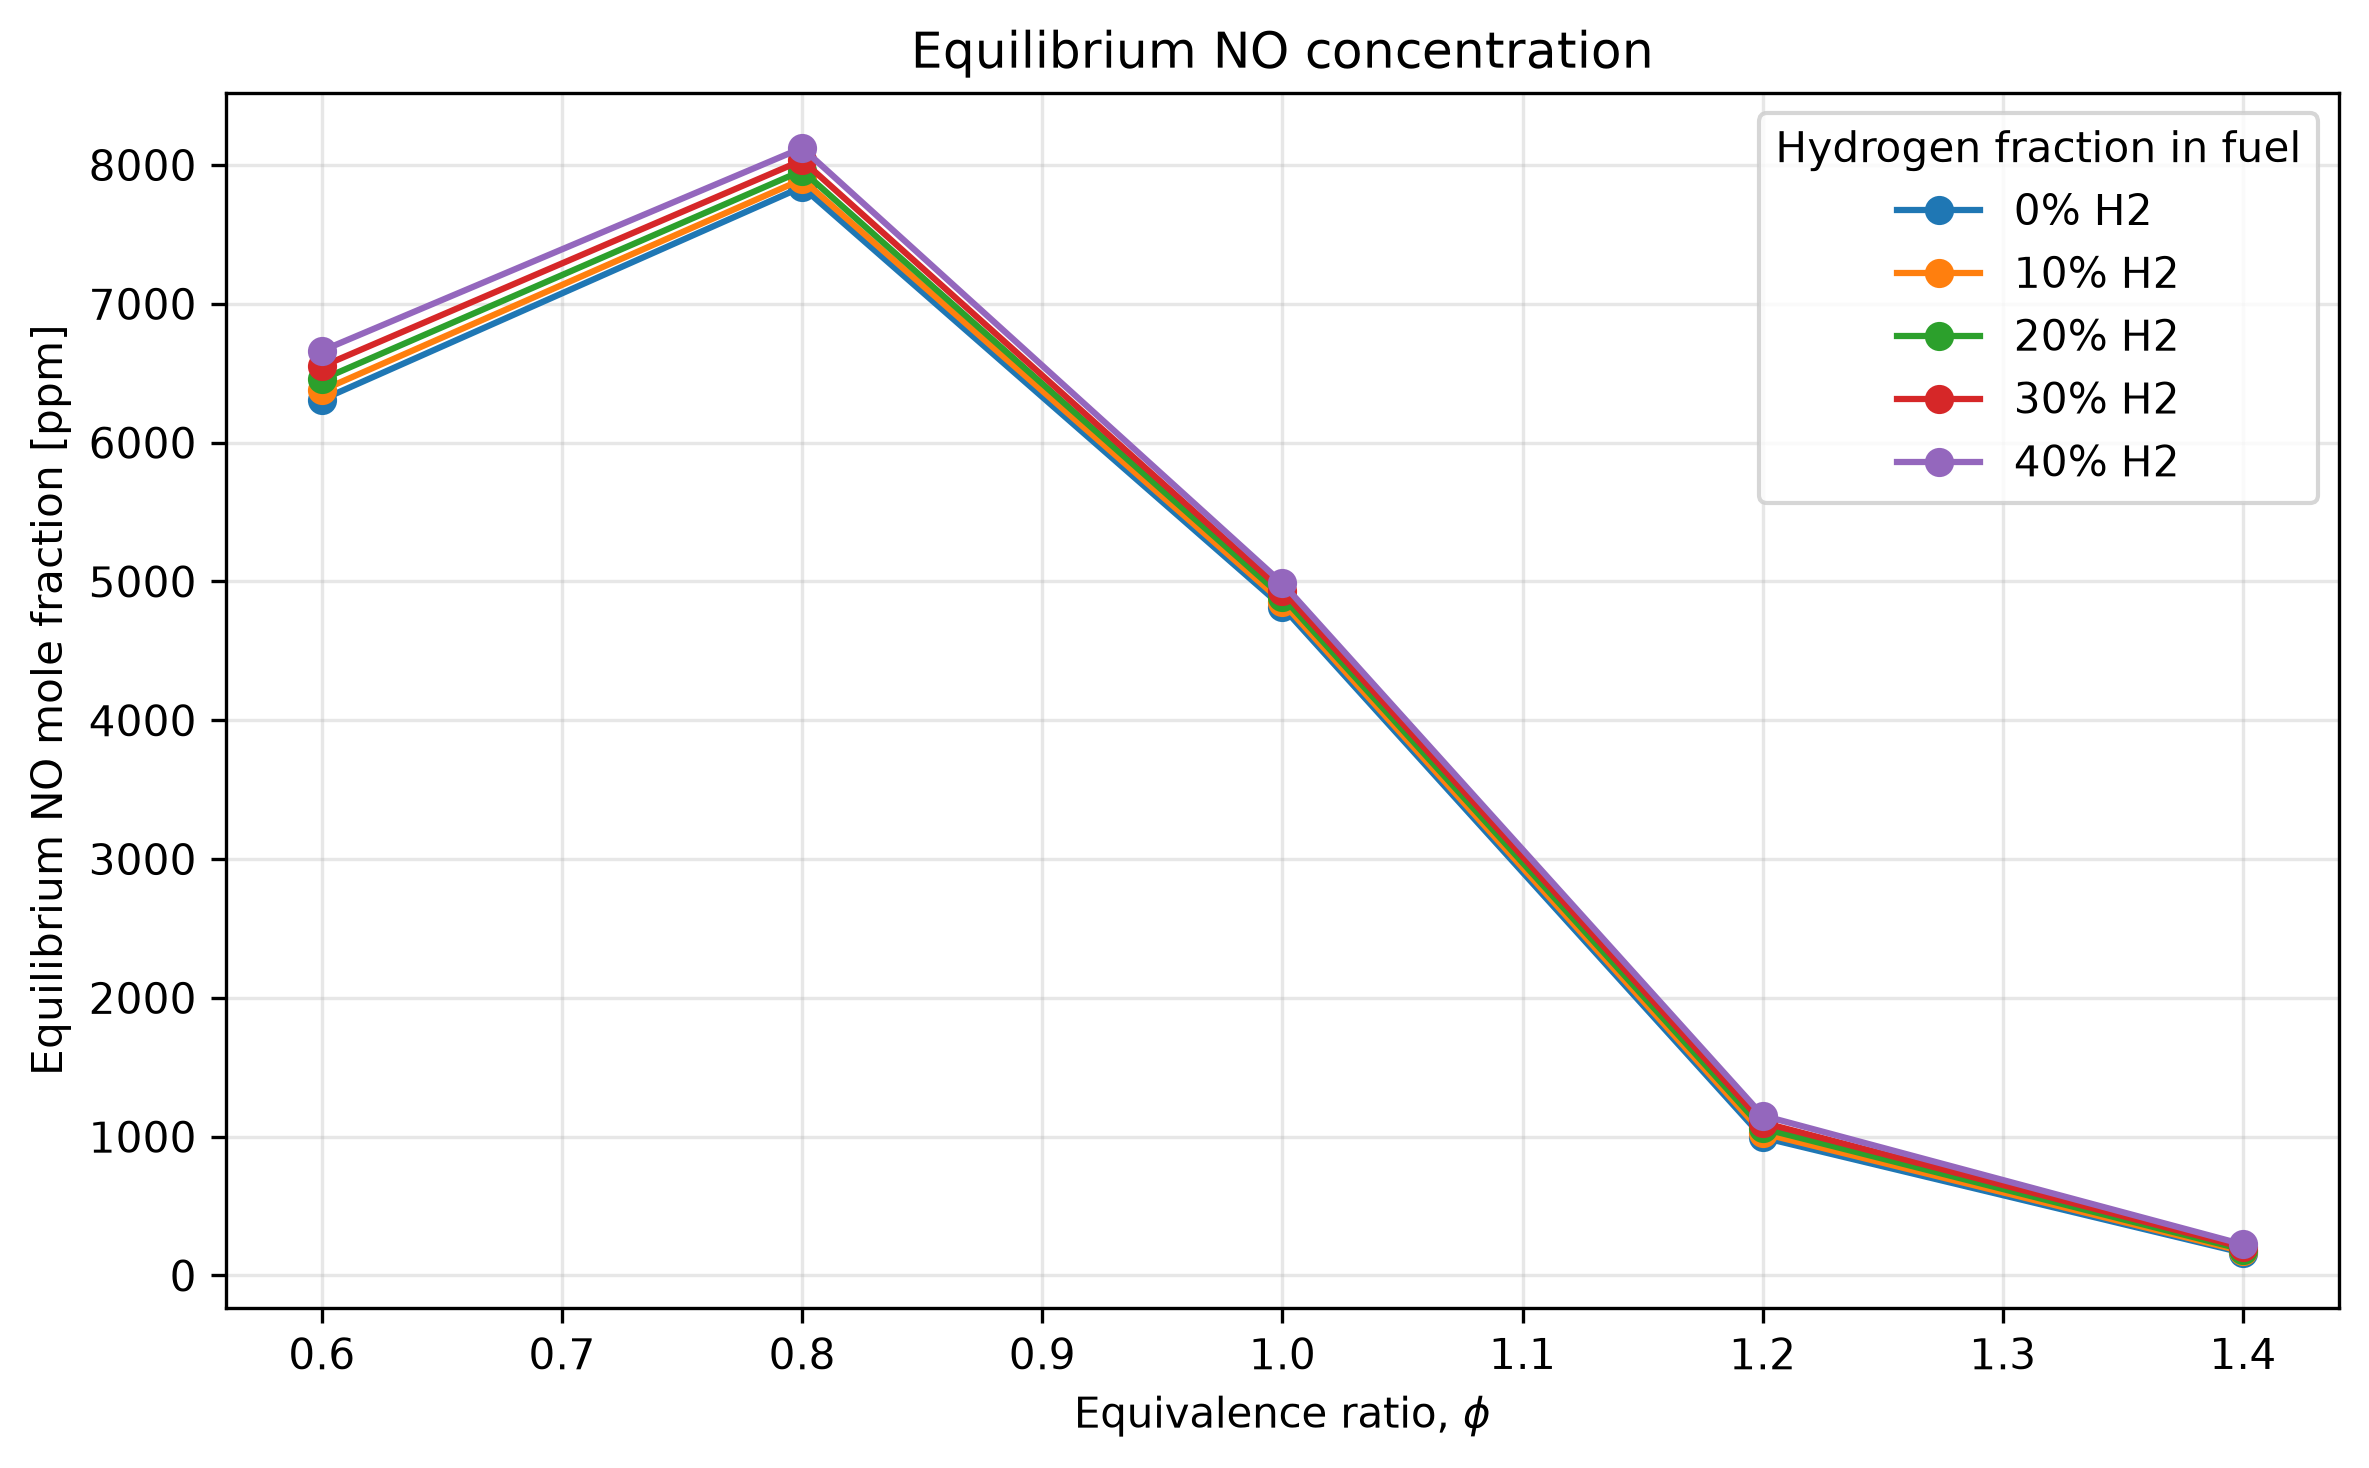
\includegraphics[width=\textwidth]{no_vs_phi.png}
    \caption{Equilibrium \ce{NO}.}
  \end{subfigure}\hfill
  \begin{subfigure}{0.49\textwidth}
    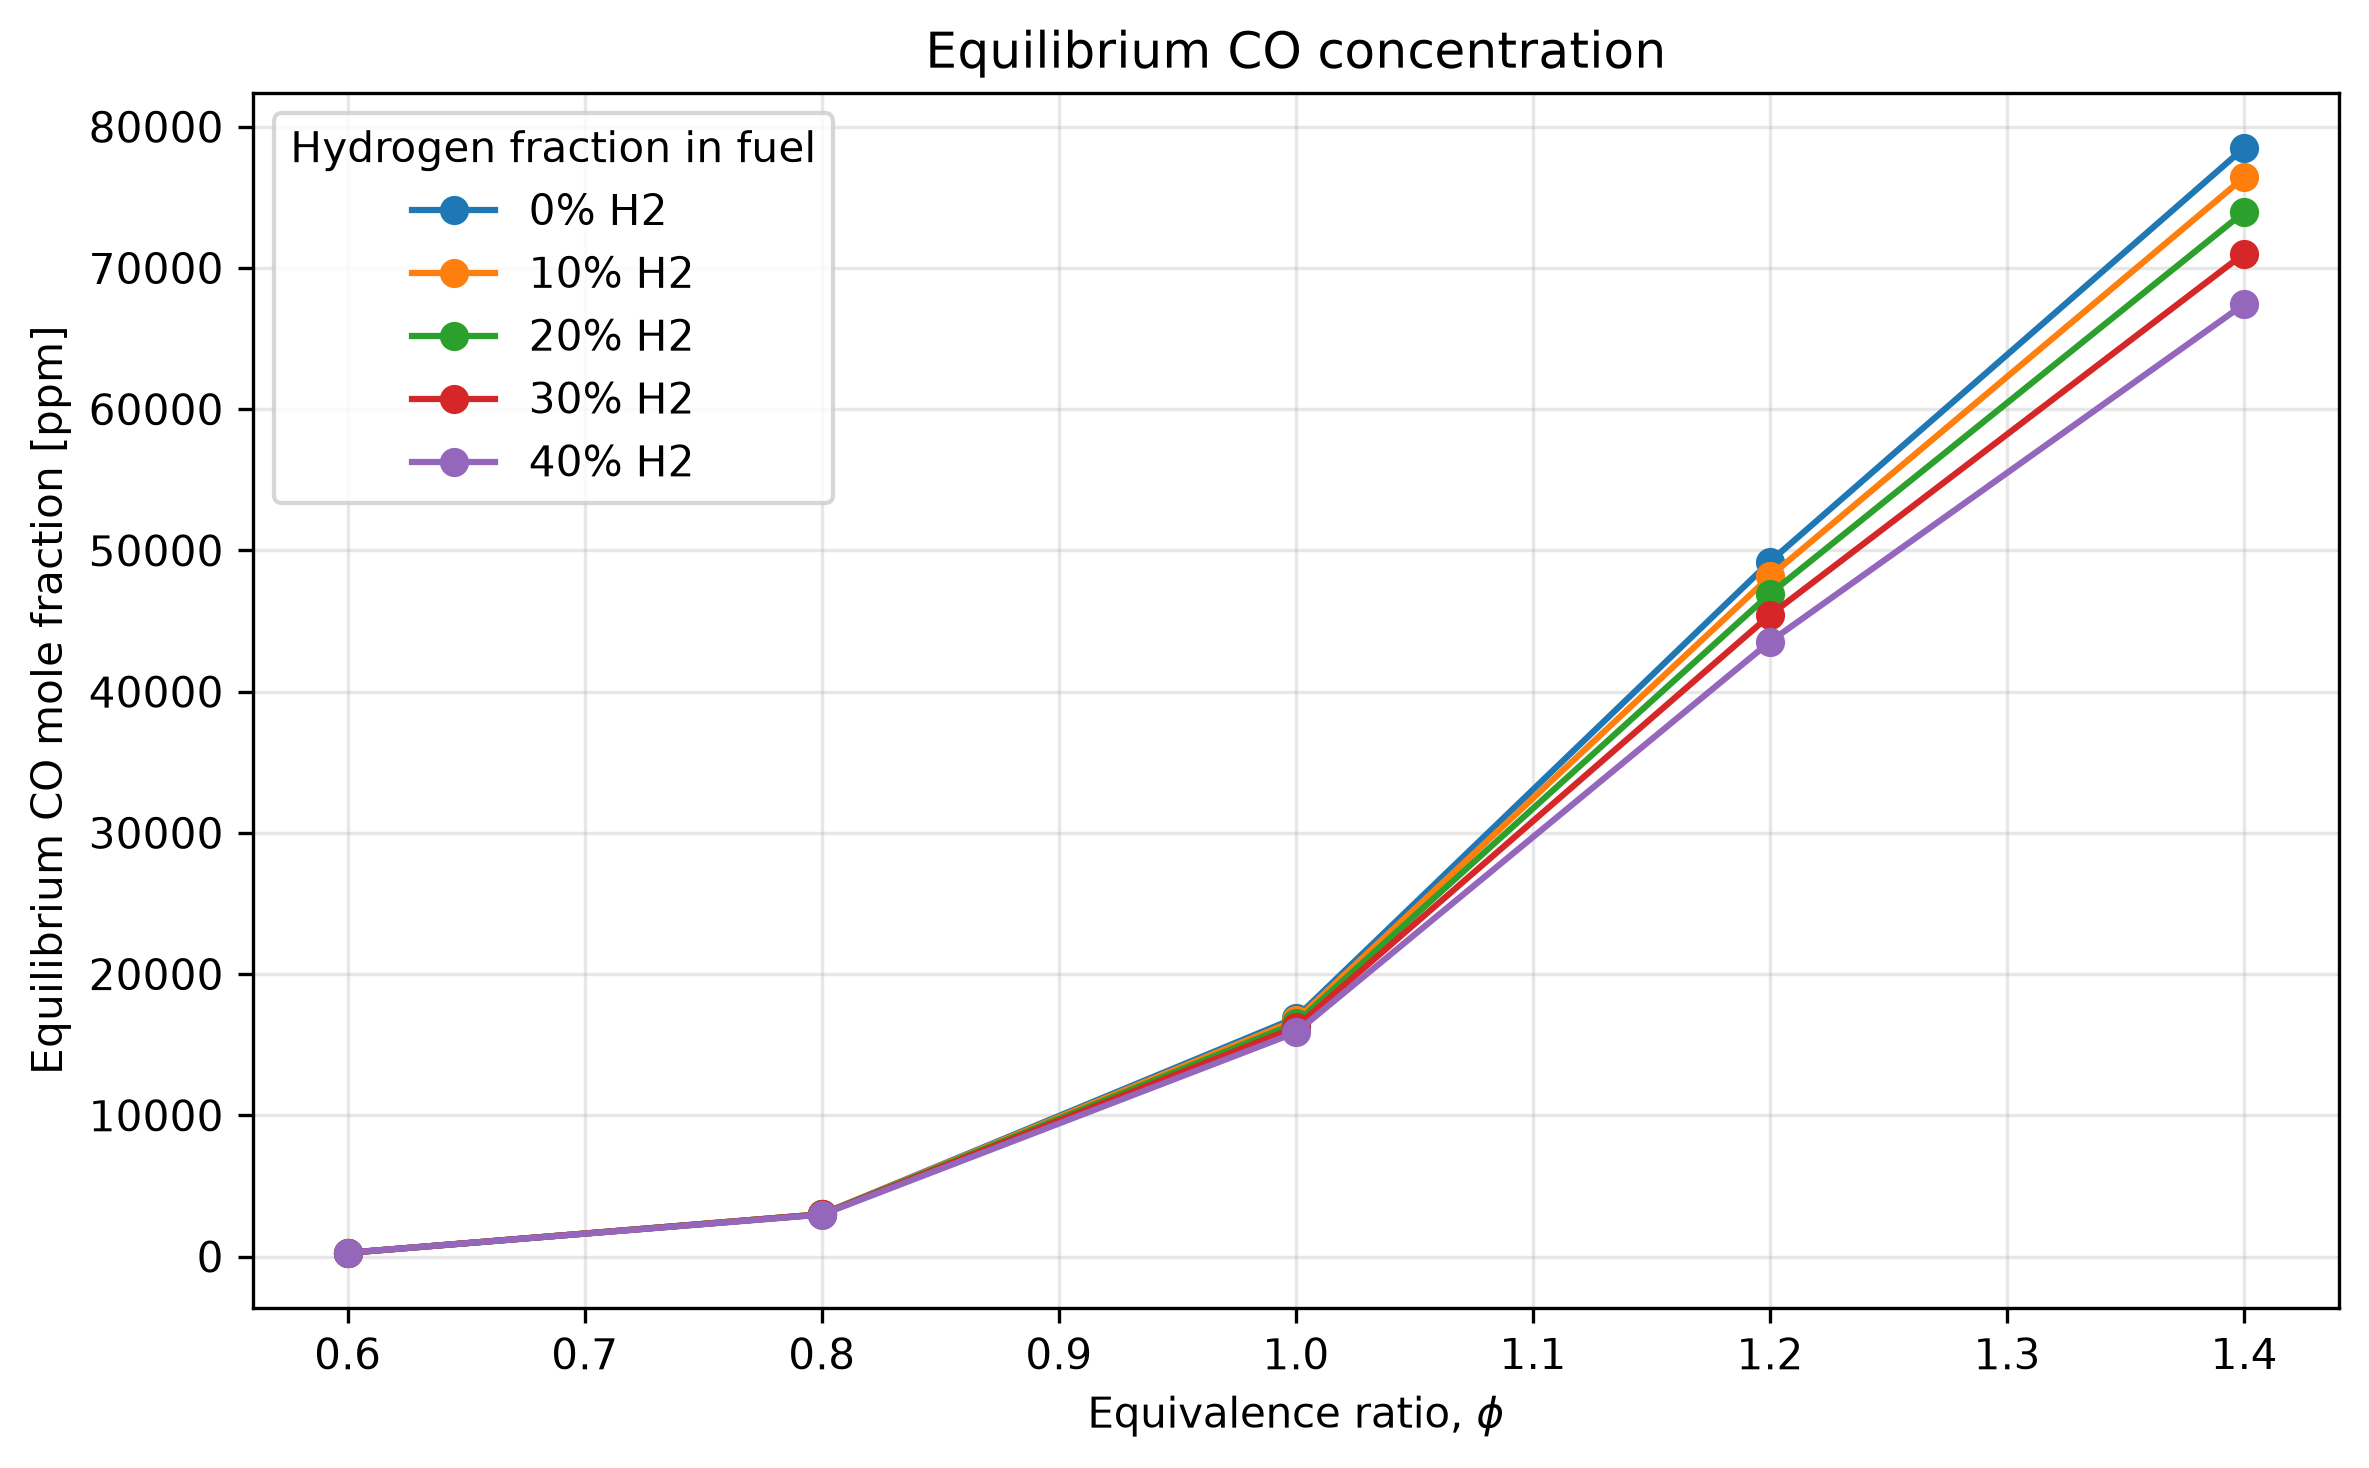
\includegraphics[width=\textwidth]{co_vs_phi.png}
    \caption{Equilibrium \ce{CO}.}
  \end{subfigure}
  \caption{Equilibrium pollutant mole fractions versus equivalence ratio at
           $T_0=\SI{900}{\kelvin}$ and $p=\SI{10}{\atmosphere}$.}
  \label{fig:eq-species}
\end{figure}

\subsection{Nitrogen oxide formation}
The equilibrium and PSR results report \ce{NO} mole fractions from the
GRI-Mech~3.0 chemistry. Established nitrogen-chemistry pathways in combustion
are reviewed by \citet{millerbowman1989}. The present study does not perform
reaction-path, rate-of-production or sensitivity analysis, so it reports only
the overall \ce{NO} trends predicted by the selected mechanism. These values
are not certified engine-emission indices.

\subsection{Autoignition delay}
The ignition-delay results show a strong temperature dependence
(Figure~\ref{fig:ign}). At $\phi=1.0$ and $p=\SI{10}{\atmosphere}$,
methane--air decreases from \SI{601.98}{\milli\second} at
$T_0=\SI{900}{\kelvin}$ to \SI{17.34}{\milli\second} at
$T_0=\SI{1100}{\kelvin}$. The \SI{40}{\mole\percent} hydrogen blend decreases
over the same temperature range from \SI{172.58}{\milli\second} to
\SI{1.39}{\milli\second}. At $T_0=\SI{1000}{\kelvin}$, hydrogen enrichment
reduces the delay from \SI{81.99}{\milli\second} at
\SI{0}{\mole\percent} hydrogen to \SI{18.09}{\milli\second} at
\SI{10}{\mole\percent}, \SI{14.34}{\milli\second} at
\SI{20}{\mole\percent}, \SI{13.21}{\milli\second} at
\SI{30}{\mole\percent} and \SI{12.64}{\milli\second} at
\SI{40}{\mole\percent}.

At $T_0=\SI{1000}{\kelvin}$ and $\phi=1.0$, increasing pressure from
\SI{5}{\atmosphere} to \SI{20}{\atmosphere} shortens the methane--air
ignition delay from \SI{178.55}{\milli\second} to
\SI{39.61}{\milli\second}. For \SI{20}{\mole\percent} hydrogen the same
pressure increase reduces the delay from \SI{18.85}{\milli\second} to
\SI{9.98}{\milli\second}, and for \SI{40}{\mole\percent} hydrogen from
\SI{14.62}{\milli\second} to \SI{9.24}{\milli\second}.

The equivalence-ratio sweep at $T_0=\SI{1000}{\kelvin}$ and
$p=\SI{10}{\atmosphere}$ shows different behaviour across fuel blends
(Figure~\ref{fig:ign-phi}). Methane--air lengthens monotonically across the
tested range, from \SI{71.76}{\milli\second} at $\phi=0.6$ to
\SI{93.52}{\milli\second} at $\phi=1.4$. The hydrogen-enriched cases shorten
as the mixture is enriched over the same range: the \SI{20}{\mole\percent}
case changes from \SI{18.41}{\milli\second} to
\SI{12.37}{\milli\second}, and the \SI{40}{\mole\percent} case from
\SI{16.36}{\milli\second} to \SI{10.76}{\milli\second}. These trends are
reported as outcomes of the present finite-rate simulations; detailed radical
pathway attribution would require additional reaction-path or sensitivity
analysis.

\begin{figure}[tbp]
  \centering
  \begin{subfigure}{0.78\textwidth}
    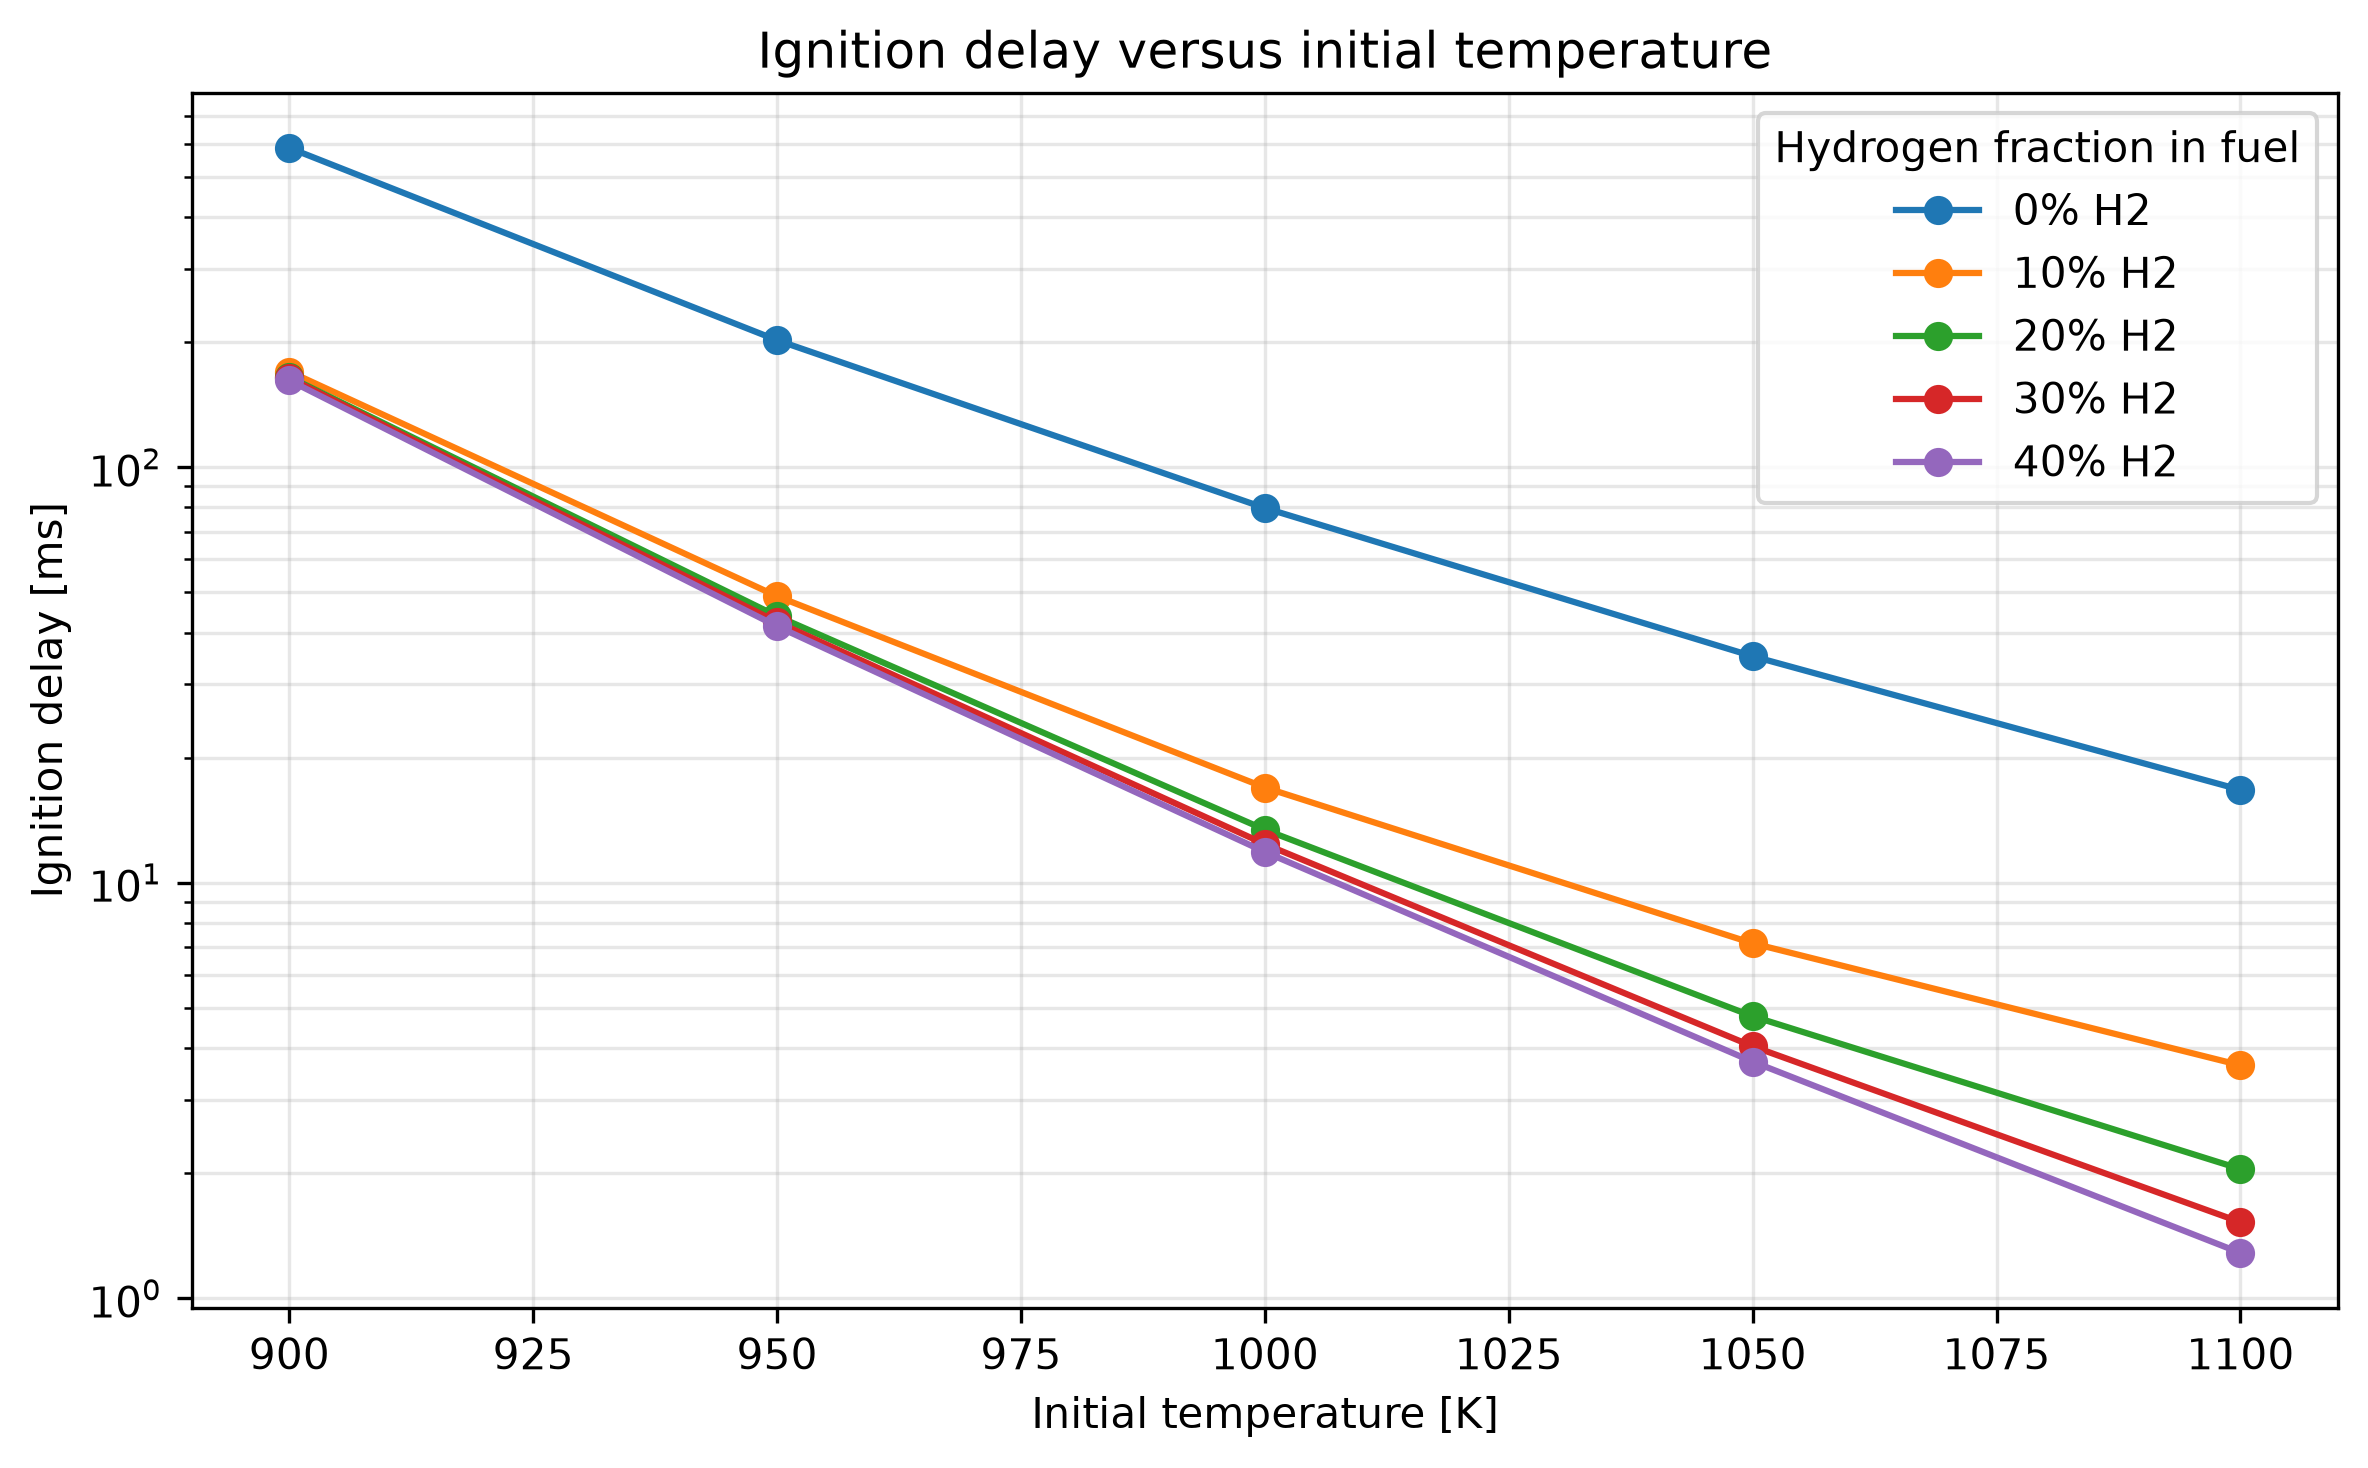
\includegraphics[width=\textwidth]{ignition_delay_vs_temperature.png}
    \caption{Versus initial temperature at $\phi=1.0$ and
             $p=\SI{10}{\atmosphere}$.}
  \end{subfigure}

  \begin{subfigure}{0.78\textwidth}
    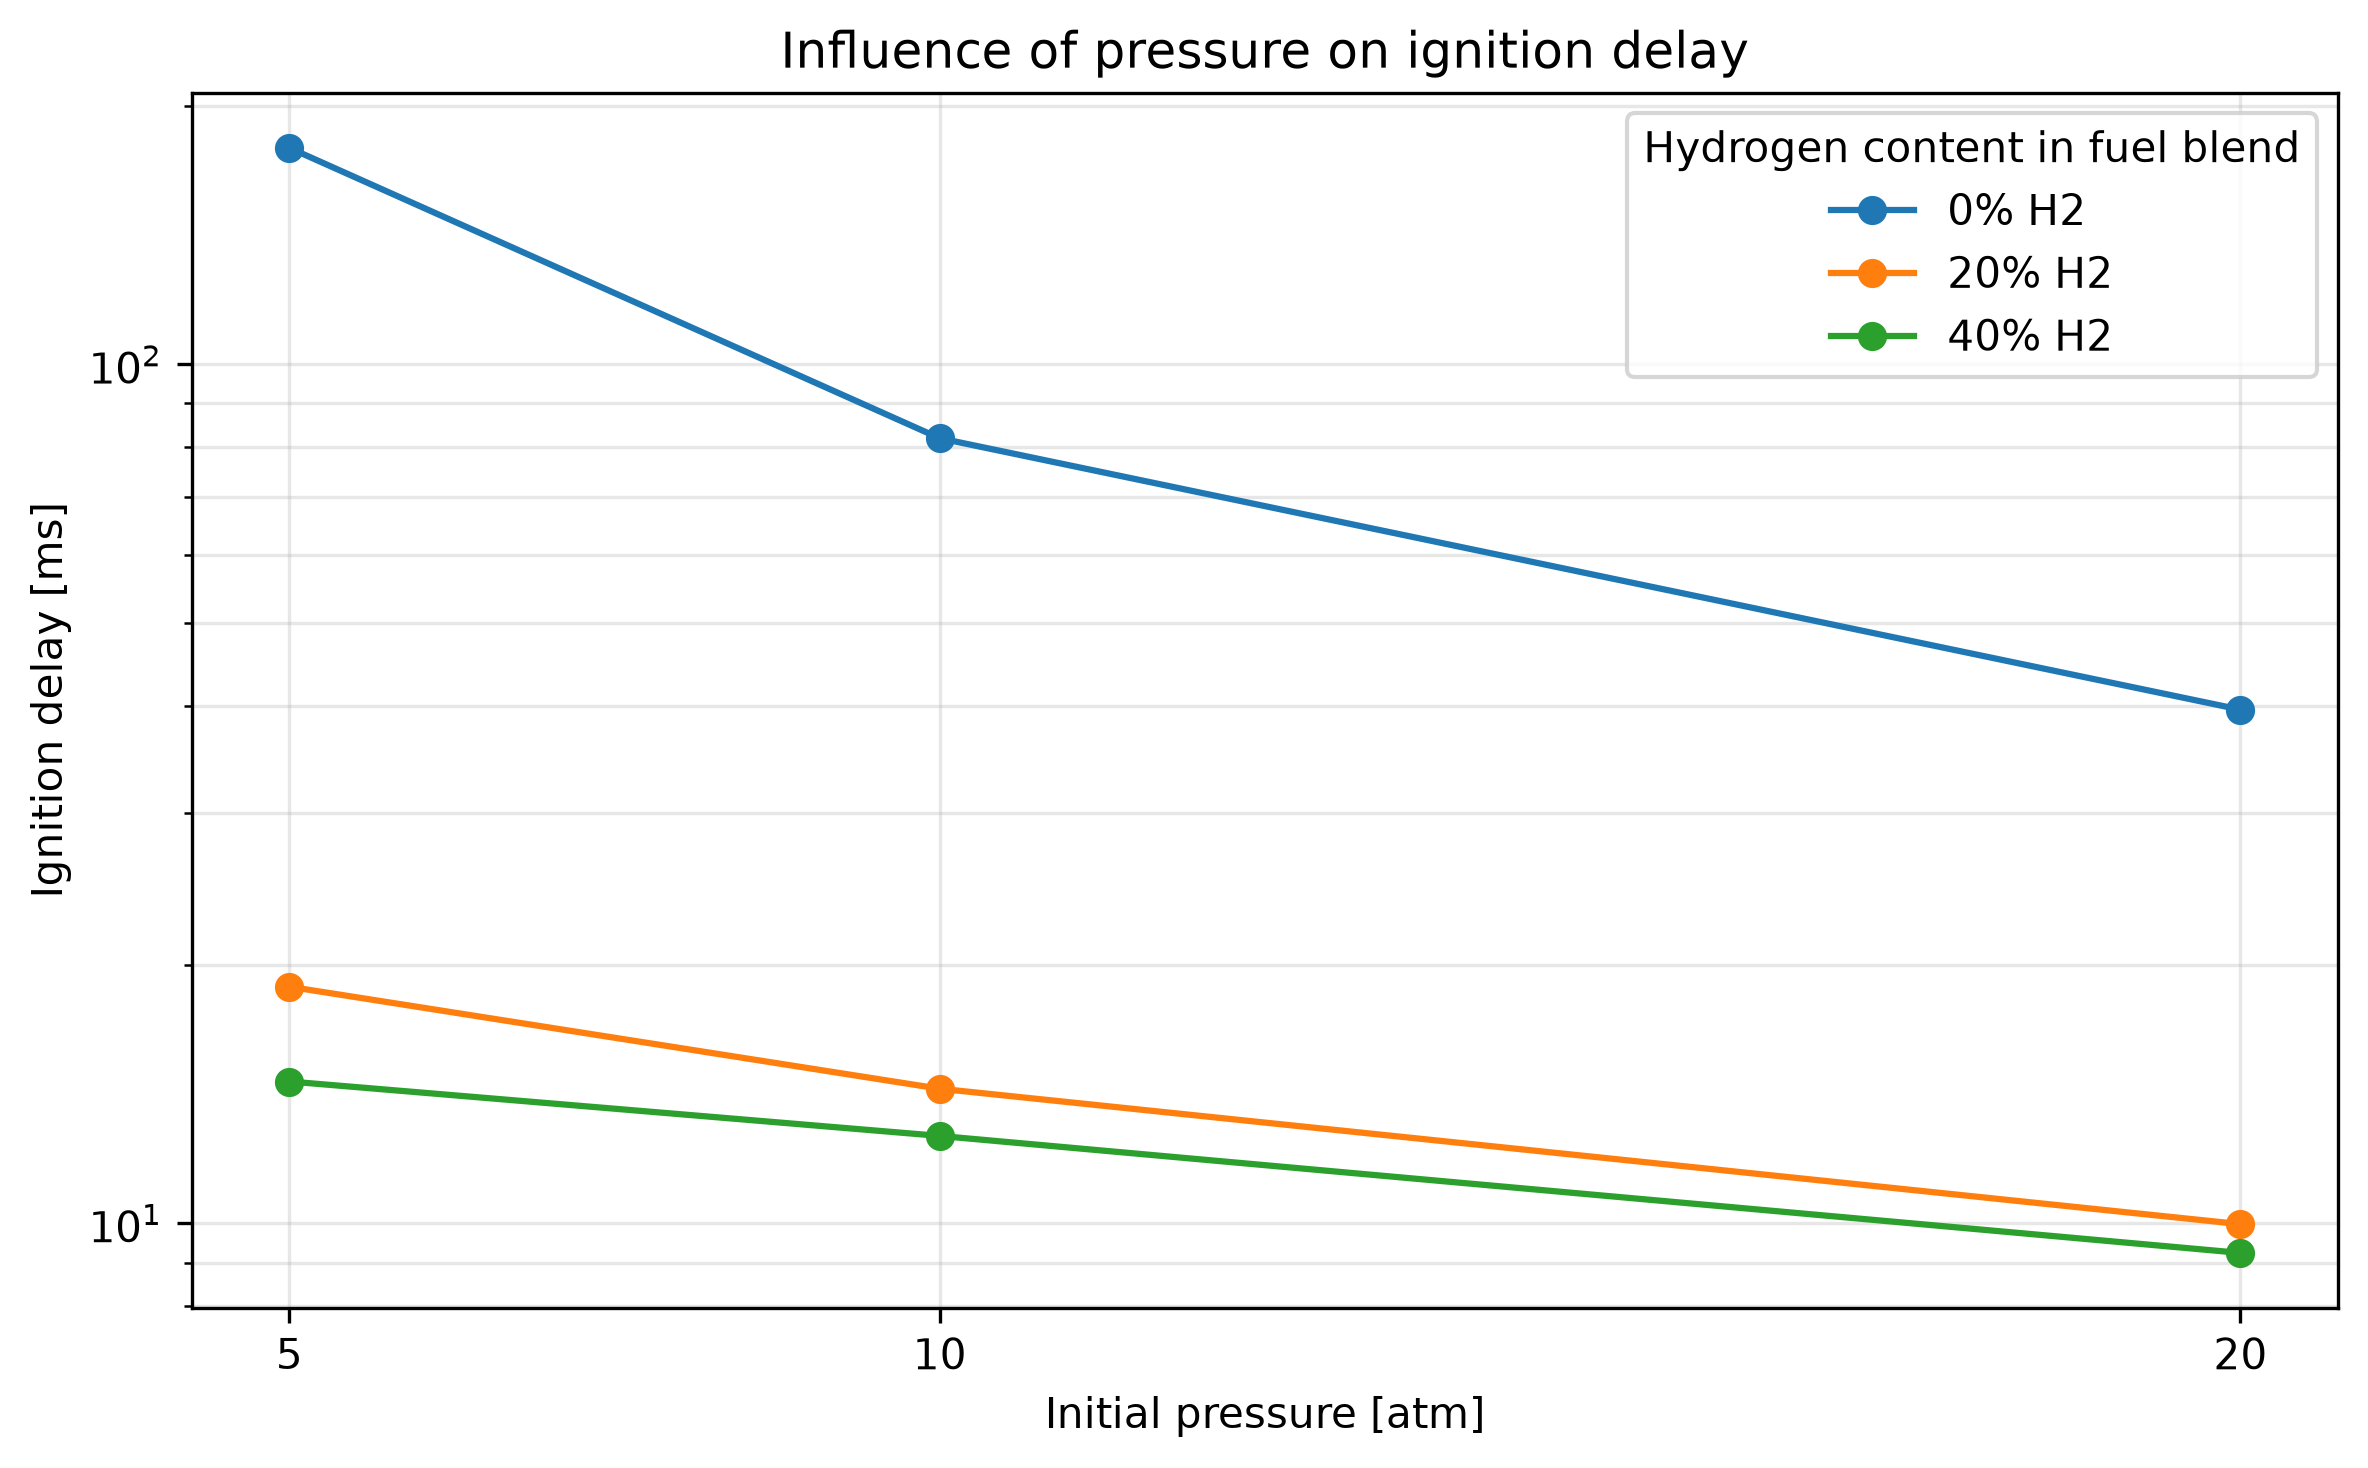
\includegraphics[width=\textwidth]{ignition_delay_vs_pressure.png}
    \caption{Versus pressure at $T_0=\SI{1000}{\kelvin}$ and $\phi=1.0$.}
  \end{subfigure}
  \caption{Autoignition delay time for the constant-pressure reactor.}
  \label{fig:ign}
\end{figure}

\begin{figure}[tbp]
  \centering
  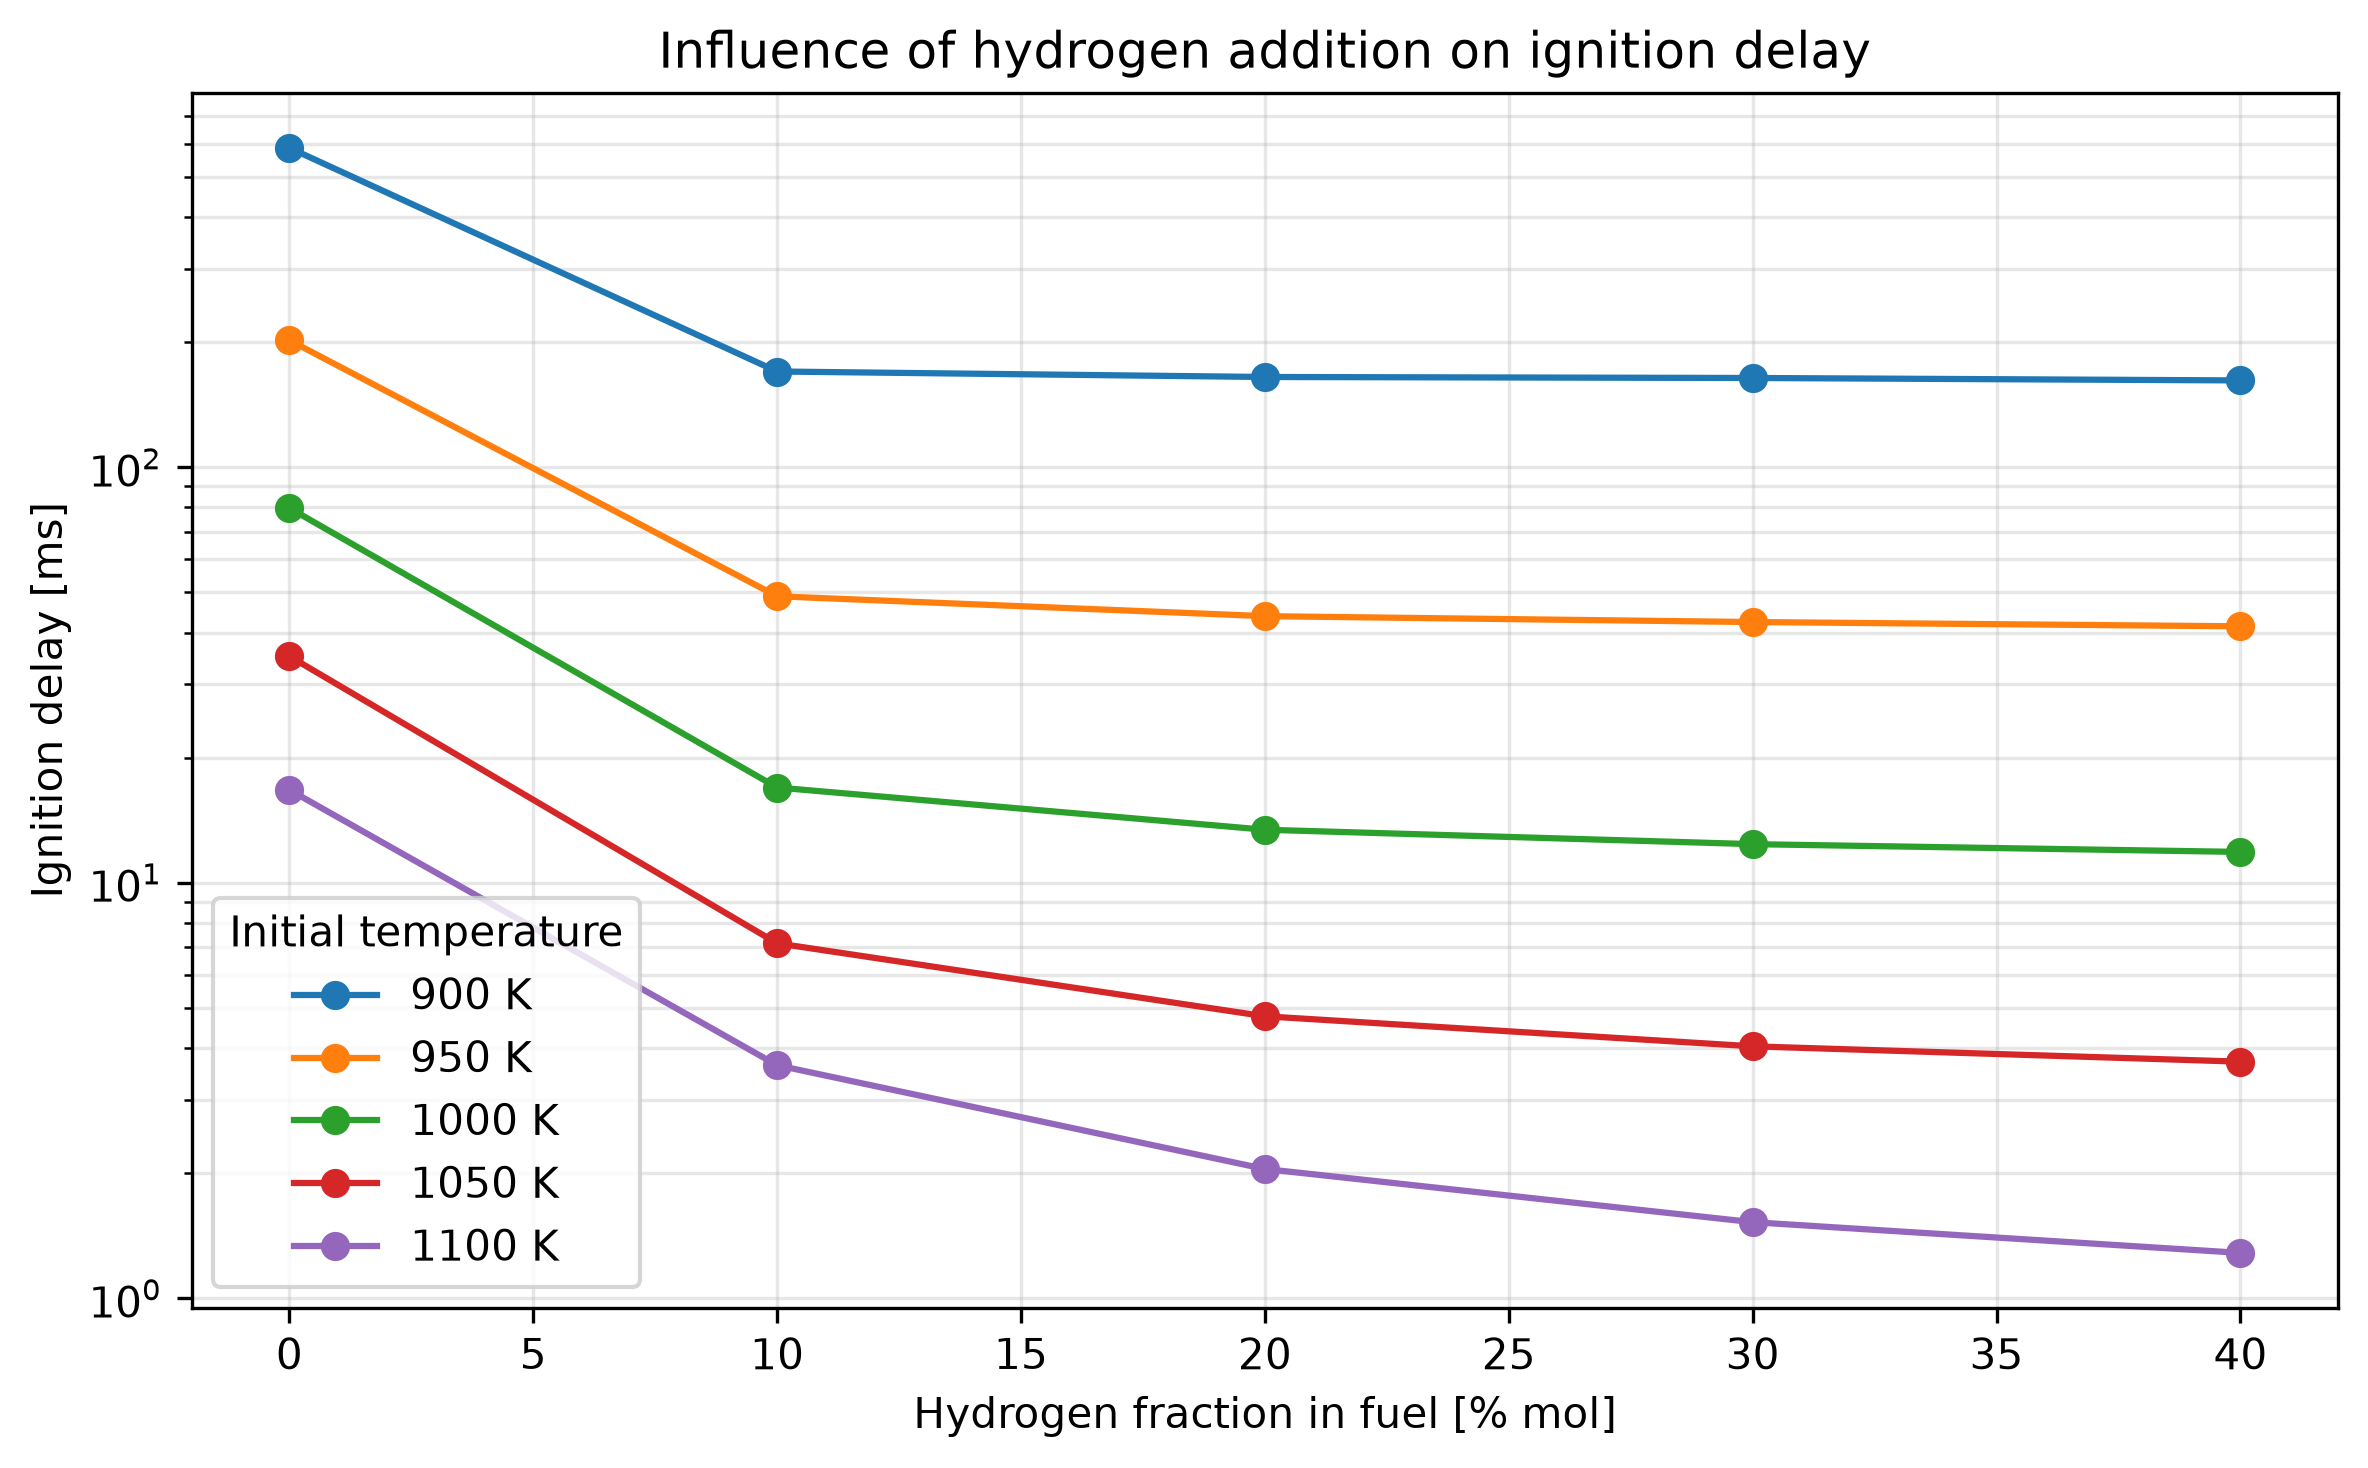
\includegraphics[width=0.82\textwidth]{ignition_delay_vs_h2_fraction.png}
  \caption{Constant-pressure ignition delay versus hydrogen fraction at
           $\phi=1.0$, $p=\SI{10}{\atmosphere}$ and
           $T_0=900$--\SI{1100}{\kelvin}. The logarithmic axis highlights
           that the strongest enrichment effect occurs between pure methane
           and the first hydrogen-containing blend in this grid.}
  \label{fig:ign-h2}
\end{figure}

\begin{figure}[tbp]
  \centering
  \begin{subfigure}{0.78\textwidth}
    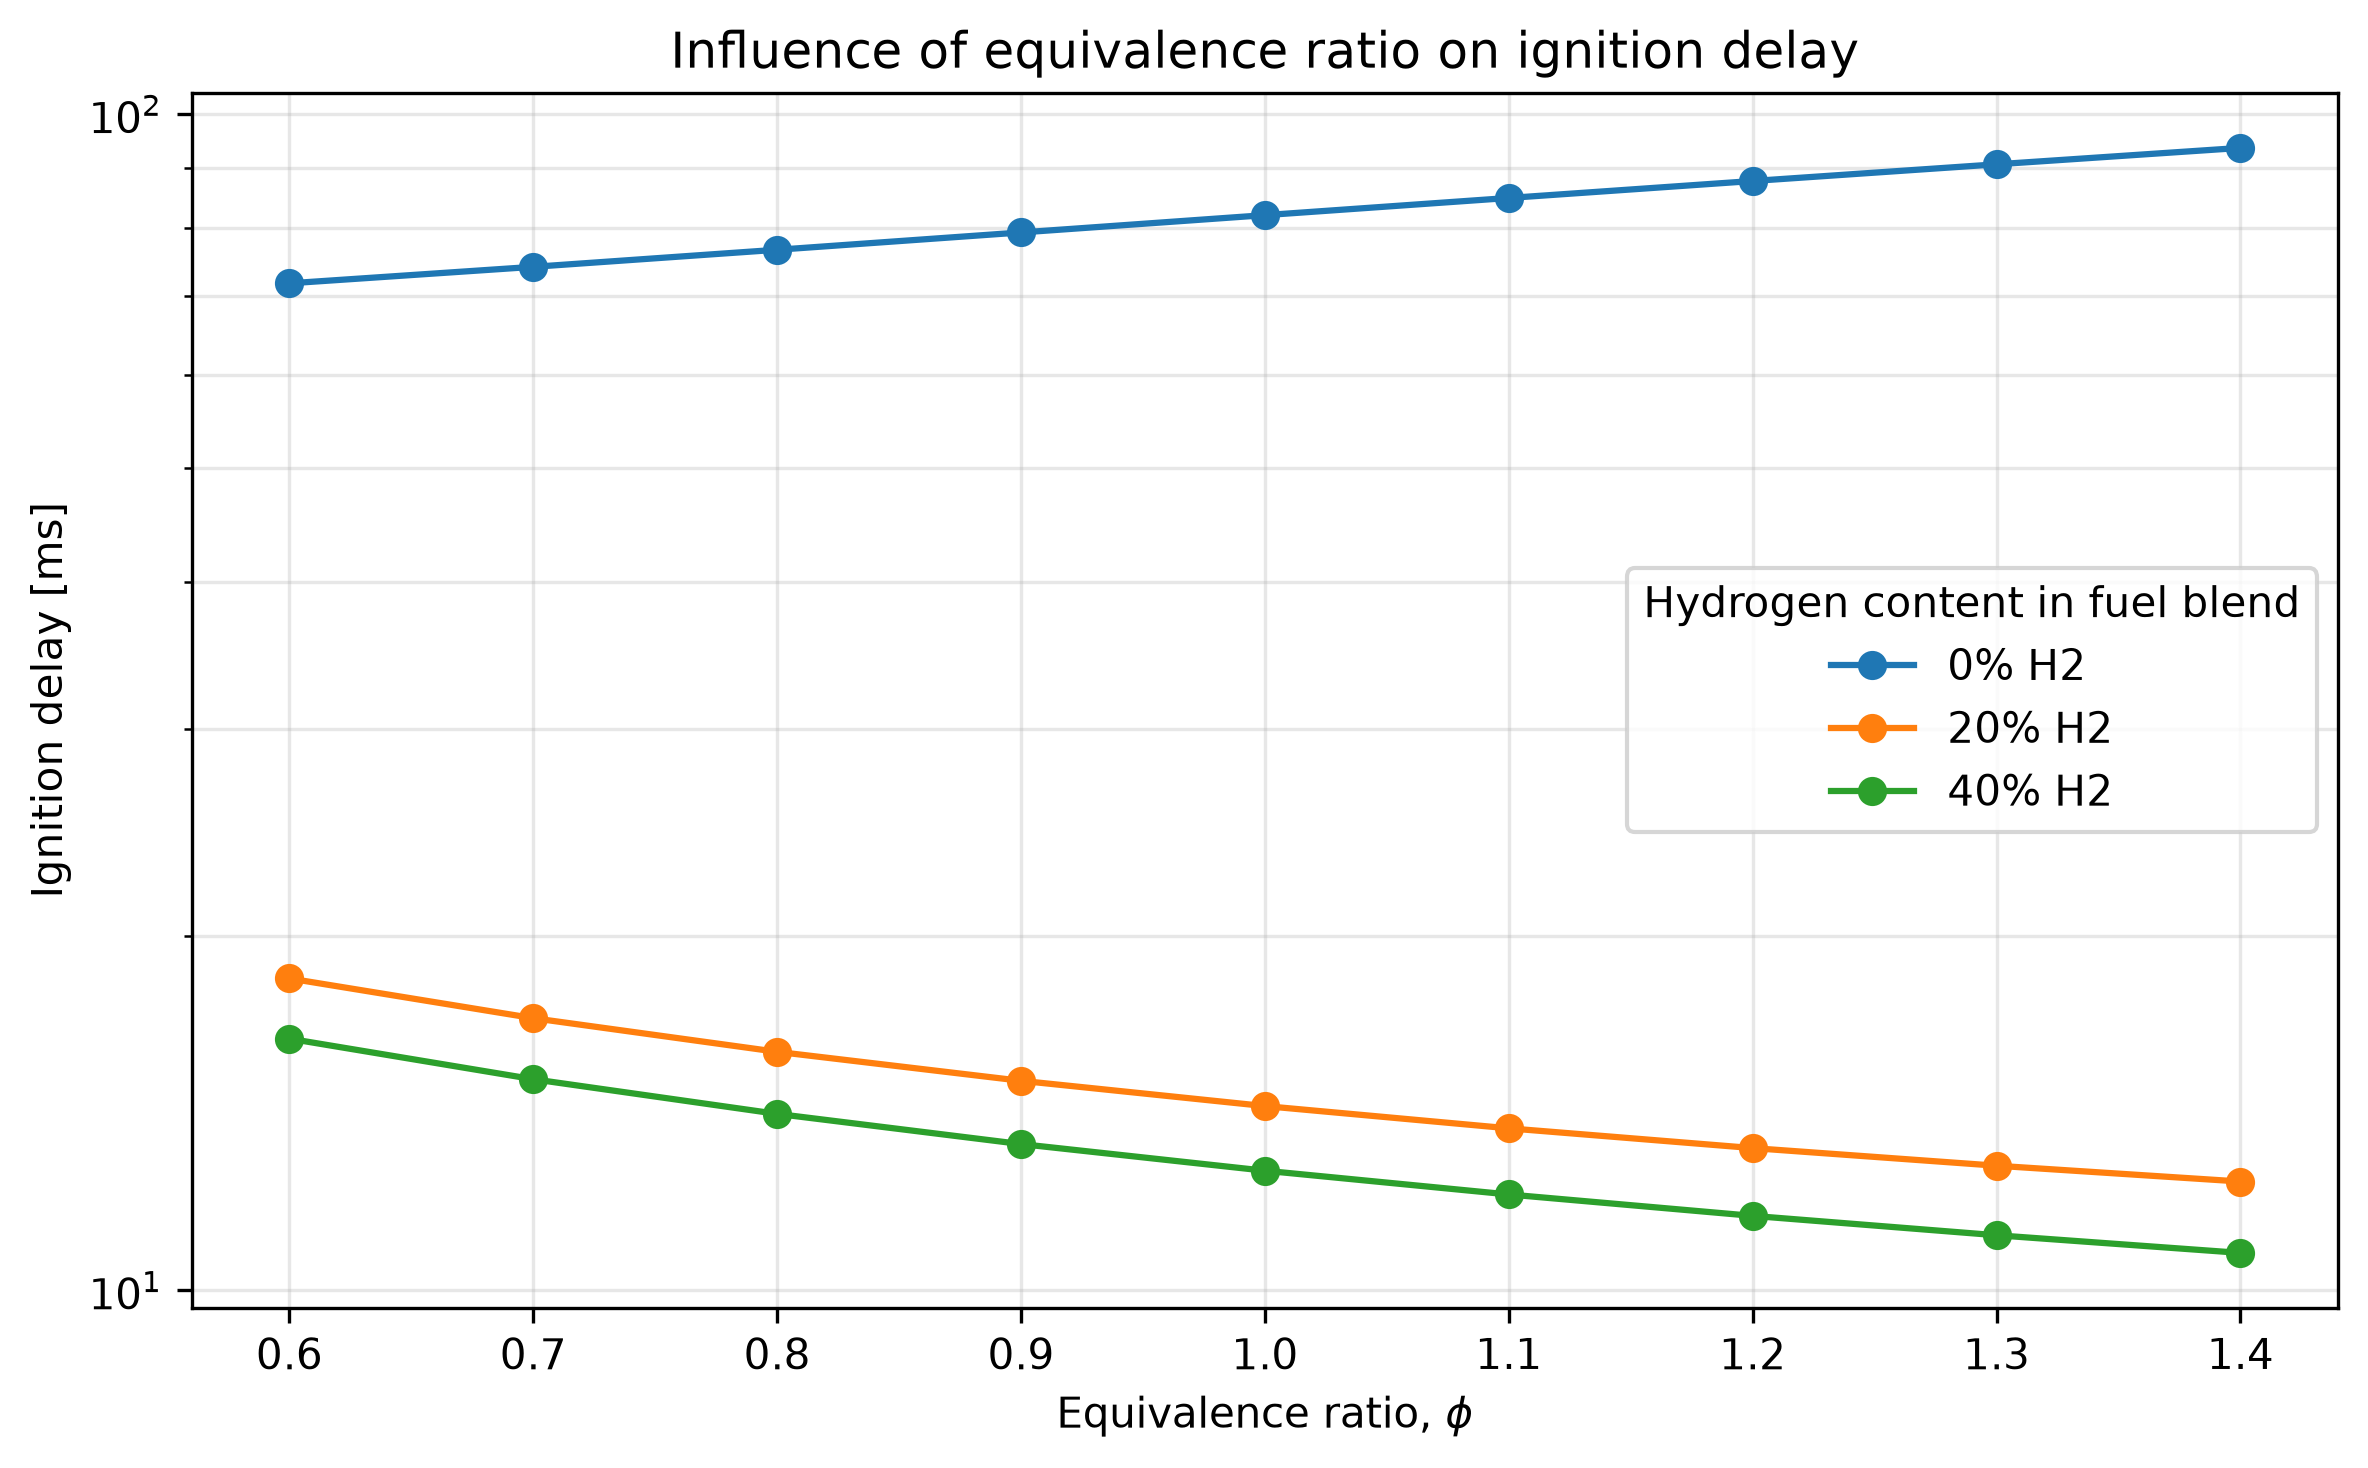
\includegraphics[width=\textwidth]{ignition_delay_vs_equivalence_ratio.png}
    \caption{Ignition delay.}
  \end{subfigure}

  \begin{subfigure}{0.78\textwidth}
    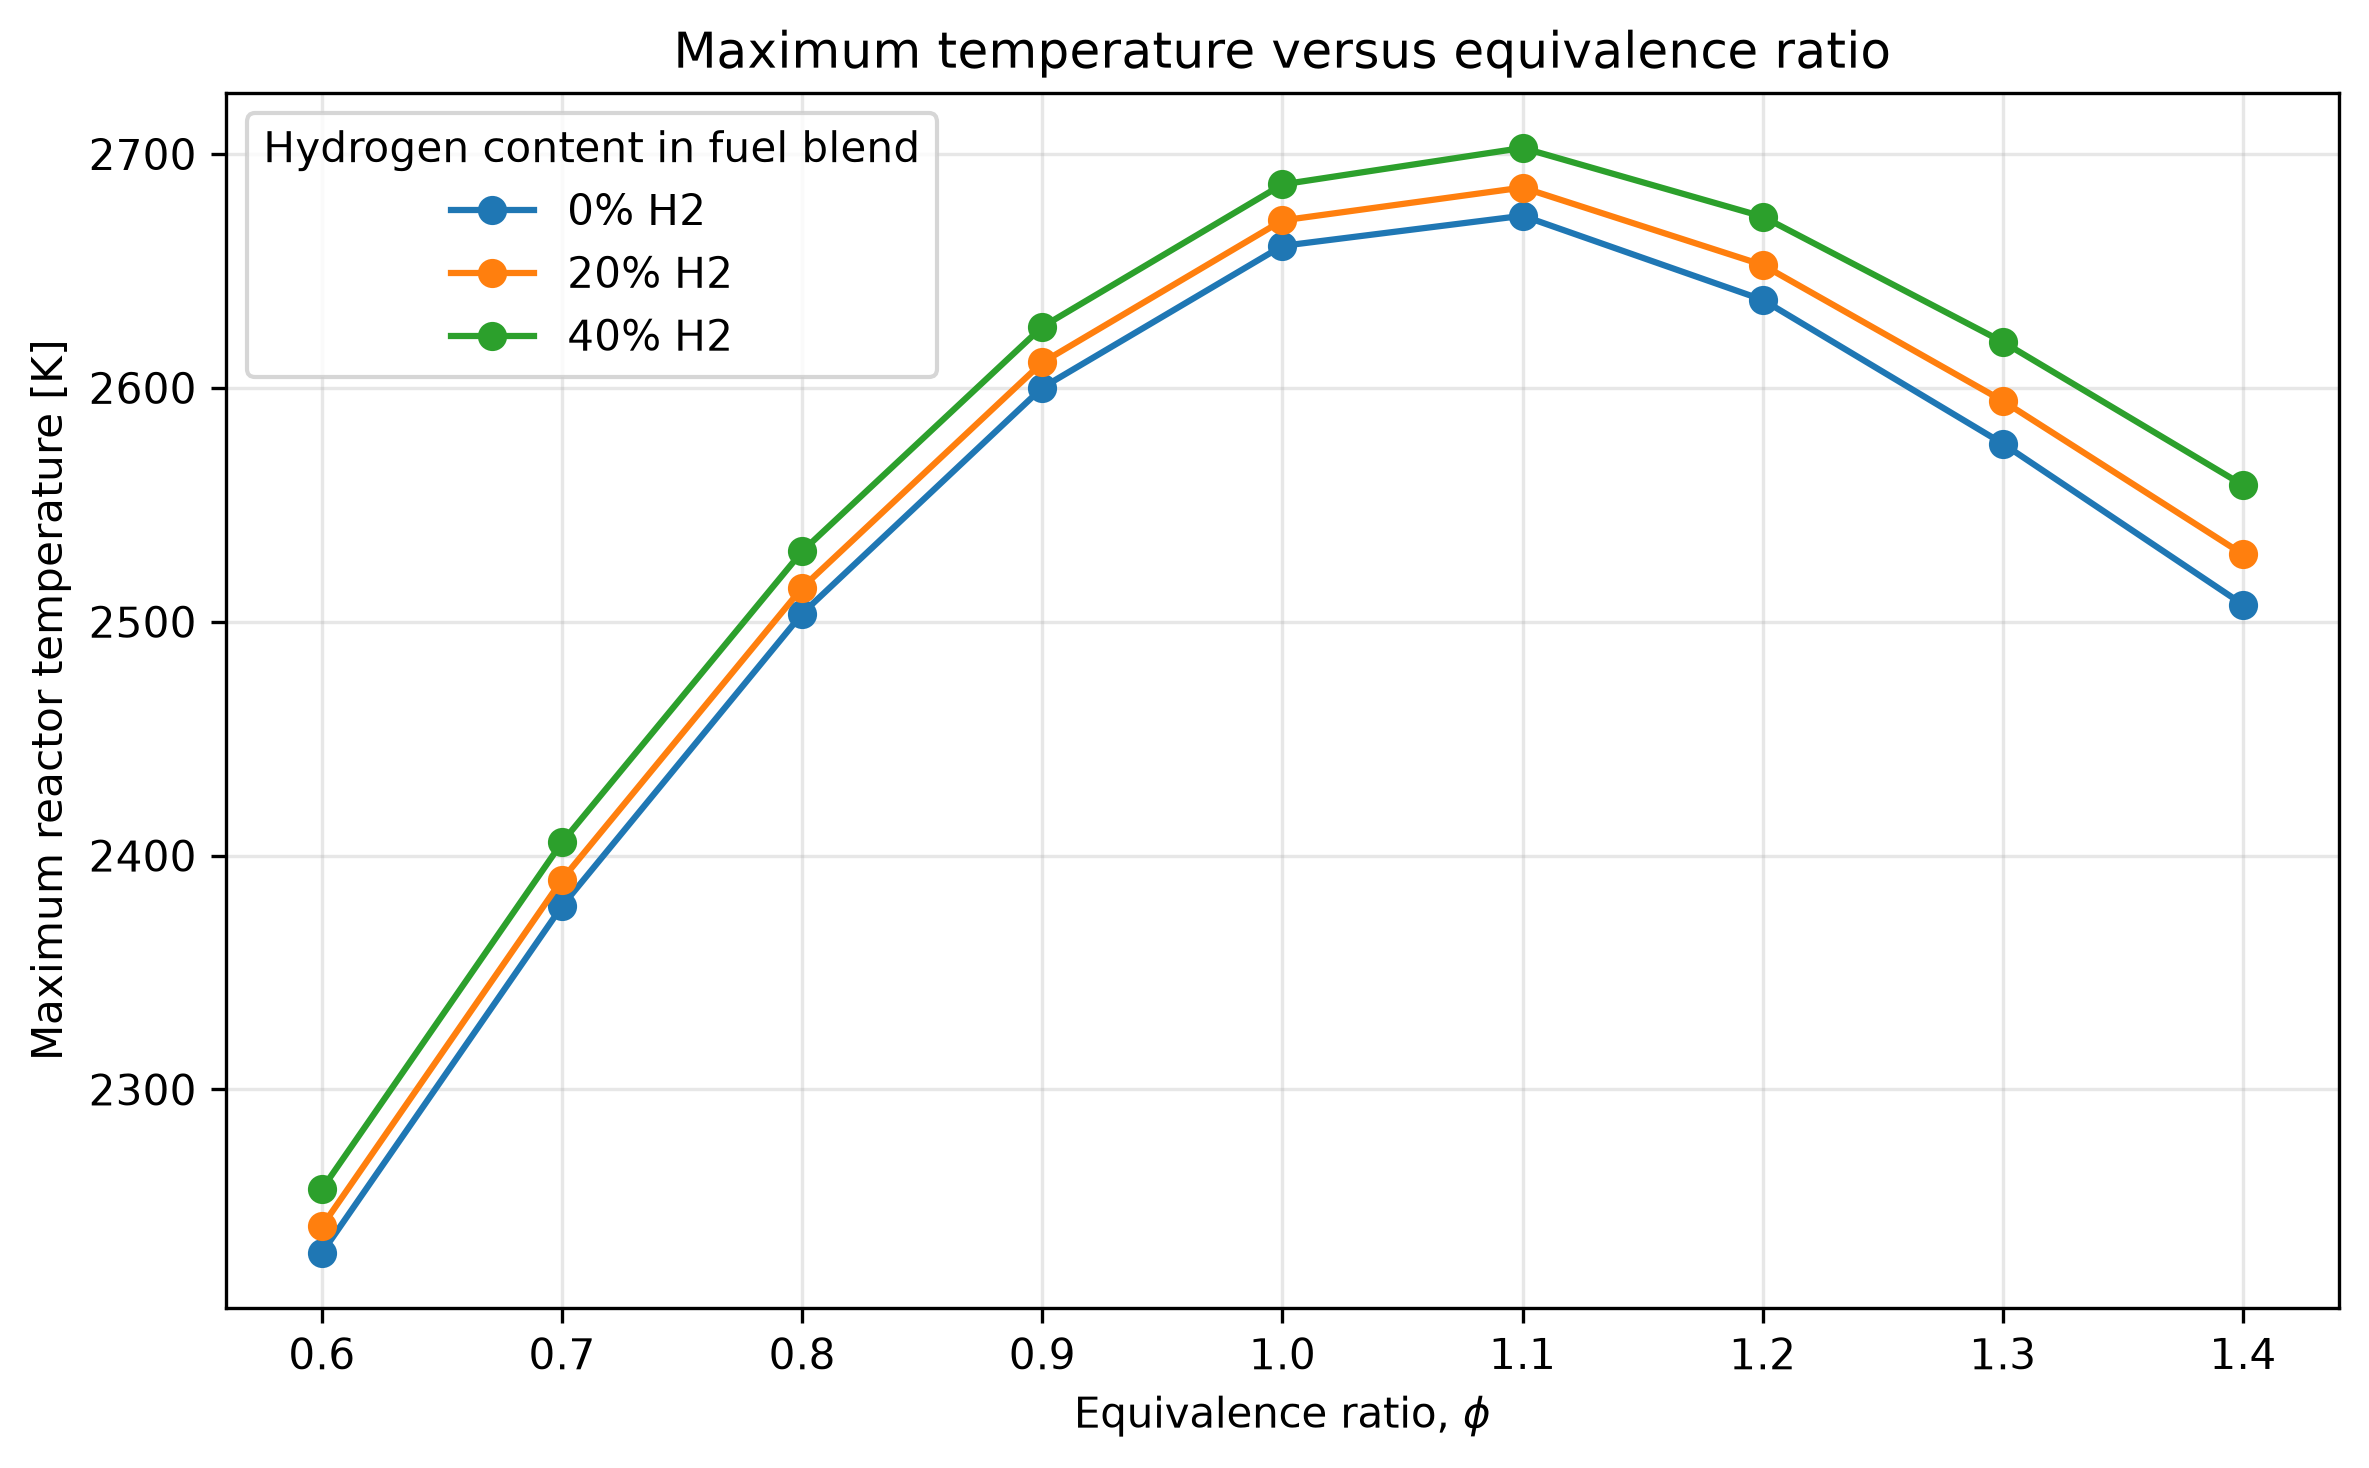
\includegraphics[width=\textwidth]{maximum_temperature_vs_equivalence_ratio.png}
    \caption{Maximum temperature.}
  \end{subfigure}
  \caption{Equivalence-ratio sweep at $T_0=\SI{1000}{\kelvin}$,
           $p=\SI{10}{\atmosphere}$ and hydrogen fractions of 0, 20 and
           \SI{40}{\mole\percent}.}
  \label{fig:ign-phi}
\end{figure}

\subsection{Two-dimensional ignition-delay map}
A supplementary ignition-delay map was computed with the same homogeneous,
adiabatic, constant-pressure reactor formulation as the one-dimensional
ignition-delay sweeps. The pressure was fixed at
$p=\SI{10}{\atmosphere}$, the initial temperature was varied from
\SI{900}{\kelvin} to \SI{1100}{\kelvin} in \SI{25}{\kelvin} increments,
and the equivalence ratio covered $\phi=0.6$--1.4 in increments of 0.1.
The hydrogen fractions were 0, 20 and \SI{40}{\mole\percent} in the fuel.
The map is intended for comparing finite-rate ignition trends across this
idealised parameter space; it is not an operational map of a real combustor,
and it does not include flow, turbulence, recirculation, wall heat loss or
geometry effects.

All 243 grid points ignited within the simulated time. Figure~\ref{fig:ign-map}
shows that the combined temperature--equivalence-ratio dependence changes
substantially with hydrogen addition. For methane--air the delay spans
\SI{14.28}{\milli\second} at $T_0=\SI{1100}{\kelvin}$, $\phi=0.6$ to
\SI{654.92}{\milli\second} at $T_0=\SI{900}{\kelvin}$, $\phi=1.4$.
At \SI{40}{\mole\percent} hydrogen, the corresponding range is
\SI{1.26}{\milli\second} at $T_0=\SI{1100}{\kelvin}$, $\phi=1.4$ to
\SI{221.04}{\milli\second} at $T_0=\SI{900}{\kelvin}$, $\phi=0.6$.
The maximum difference between the maximum-$\mathrm{d}T/\mathrm{d}t$ delay
criterion and the peak-\ce{OH} criterion is 0.156\%, so the two indicators are
consistent for this diagnostic grid.

\begin{figure}[htbp]
  \centering
  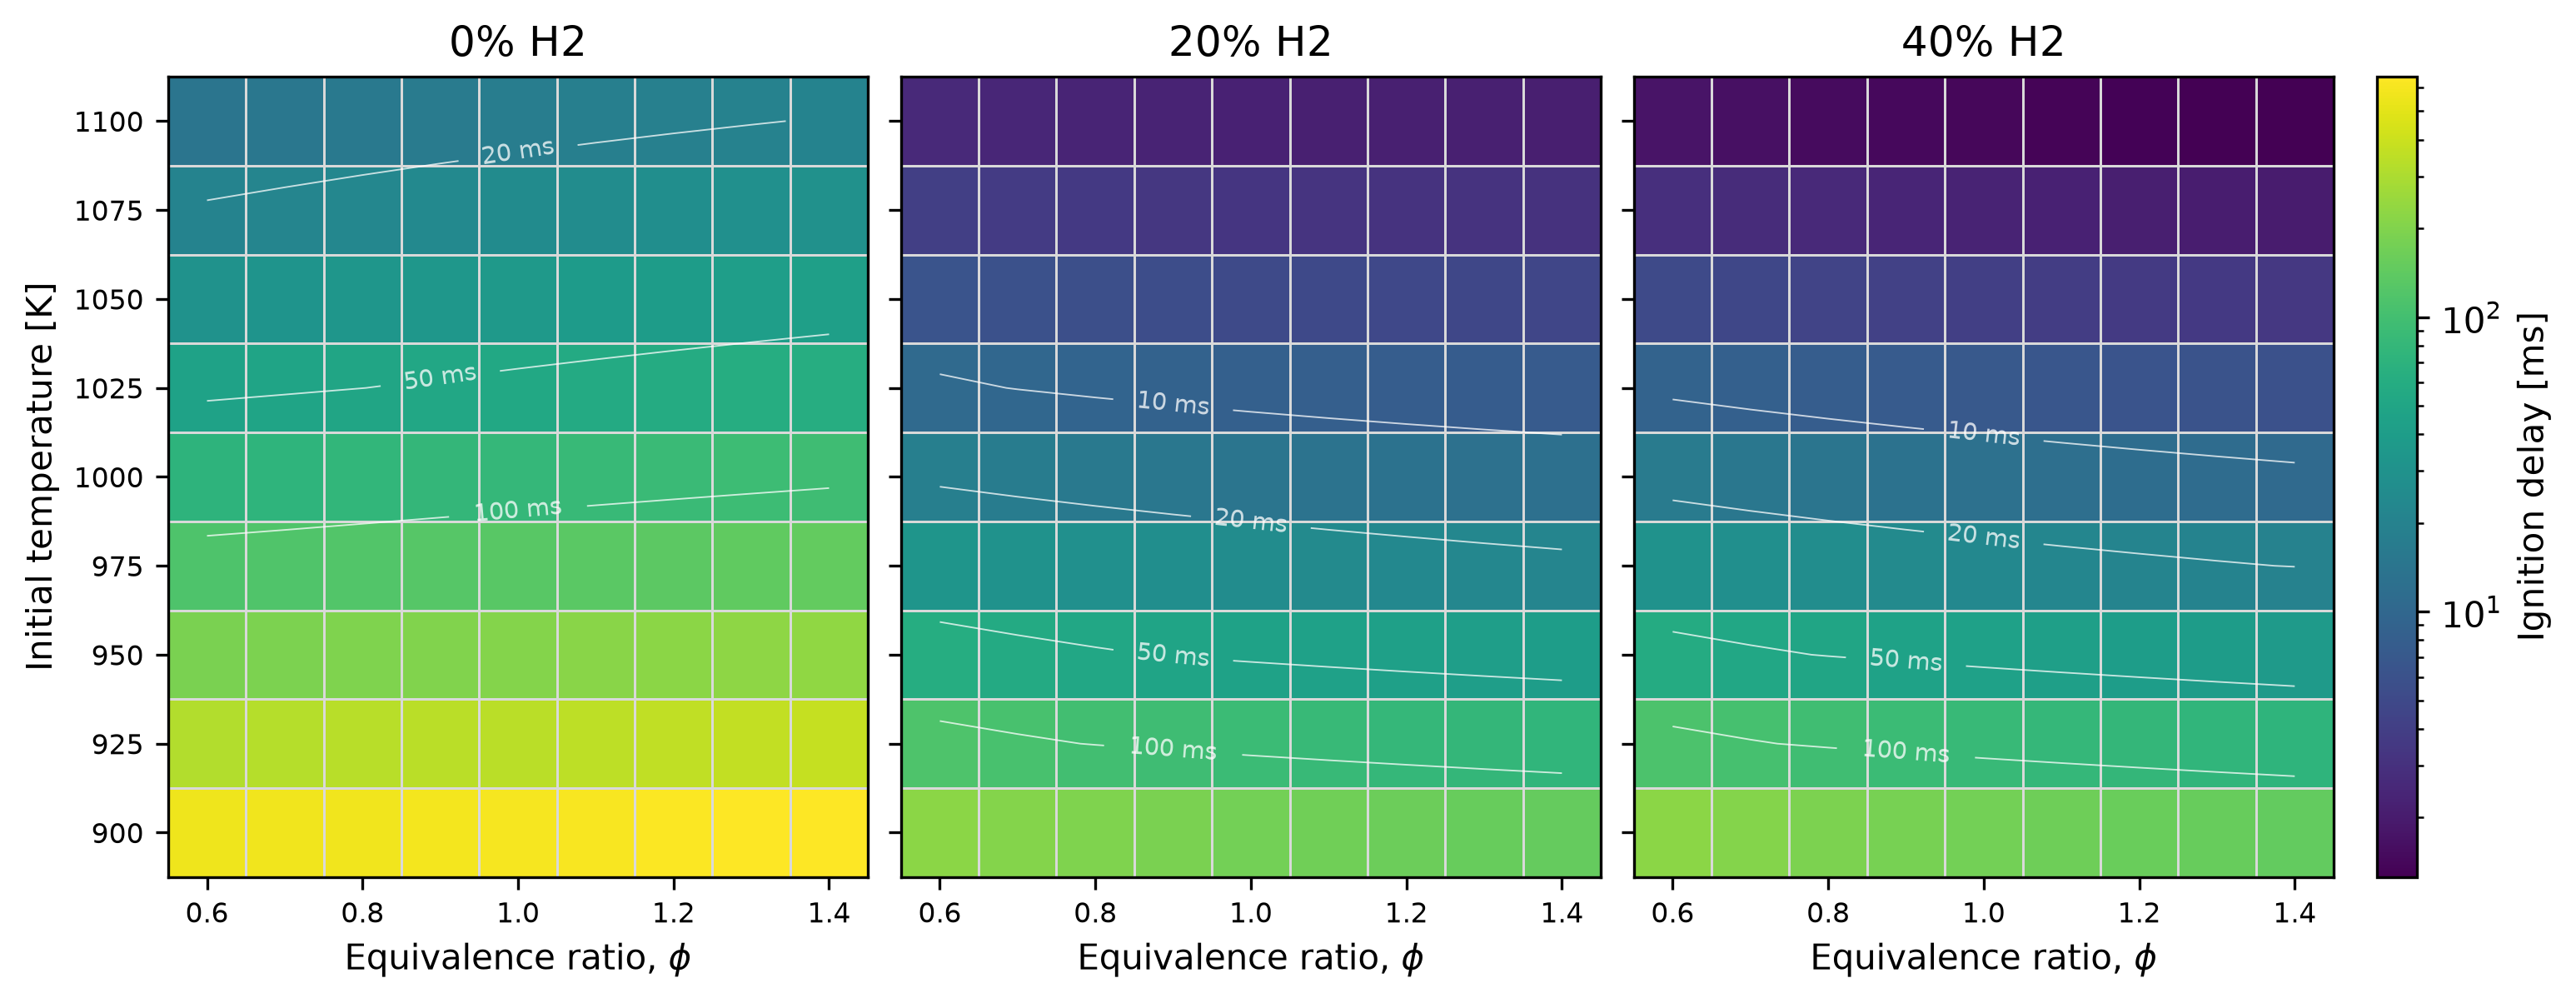
\includegraphics[width=\textwidth]{ignition_delay_map.png}
  \caption{Two-dimensional constant-pressure ignition-delay map for
           \ce{CH4}/\ce{H2}--air mixtures at $p=\SI{10}{\atmosphere}$,
           $T_0=\SI{900}{\kelvin}$--\SI{1100}{\kelvin},
           $\phi=0.6$--1.4 and fuel hydrogen fractions of 0, 20 and
           \SI{40}{\mole\percent}. Each panel uses the actual $9\times9$
           grid, the colour scale is logarithmic and common to all panels,
           and the white labels mark constant ignition-delay isolines in
           milliseconds. This is an ideal homogeneous-reactor diagnostic,
           not an operational map of a real combustion chamber.}
  \label{fig:ign-map}
\end{figure}

The ignition-delay reduction factor in Figure~\ref{fig:ign-reduction} is
computed only where both cases ignite:
\begin{equation}
  R_{\tau}
  =
  \frac{
    \tau_{\mathrm{ign},\,0\%\,\ce{H2}}
  }{
    \tau_{\mathrm{ign},\,40\%\,\ce{H2}}
  }.
\end{equation}
It ranges from 2.54 at $T_0=\SI{900}{\kelvin}$, $\phi=0.6$ to 16.28
at $T_0=\SI{1100}{\kelvin}$, $\phi=1.4$. Values greater than one mean that
the calculated ignition delay is shorter after adding \SI{40}{\mole\percent}
hydrogen to the fuel. This factor is a kinetic ignition-delay comparison
only, not an engine efficiency, performance or emissions metric.

\begin{figure}[tbp]
  \centering
  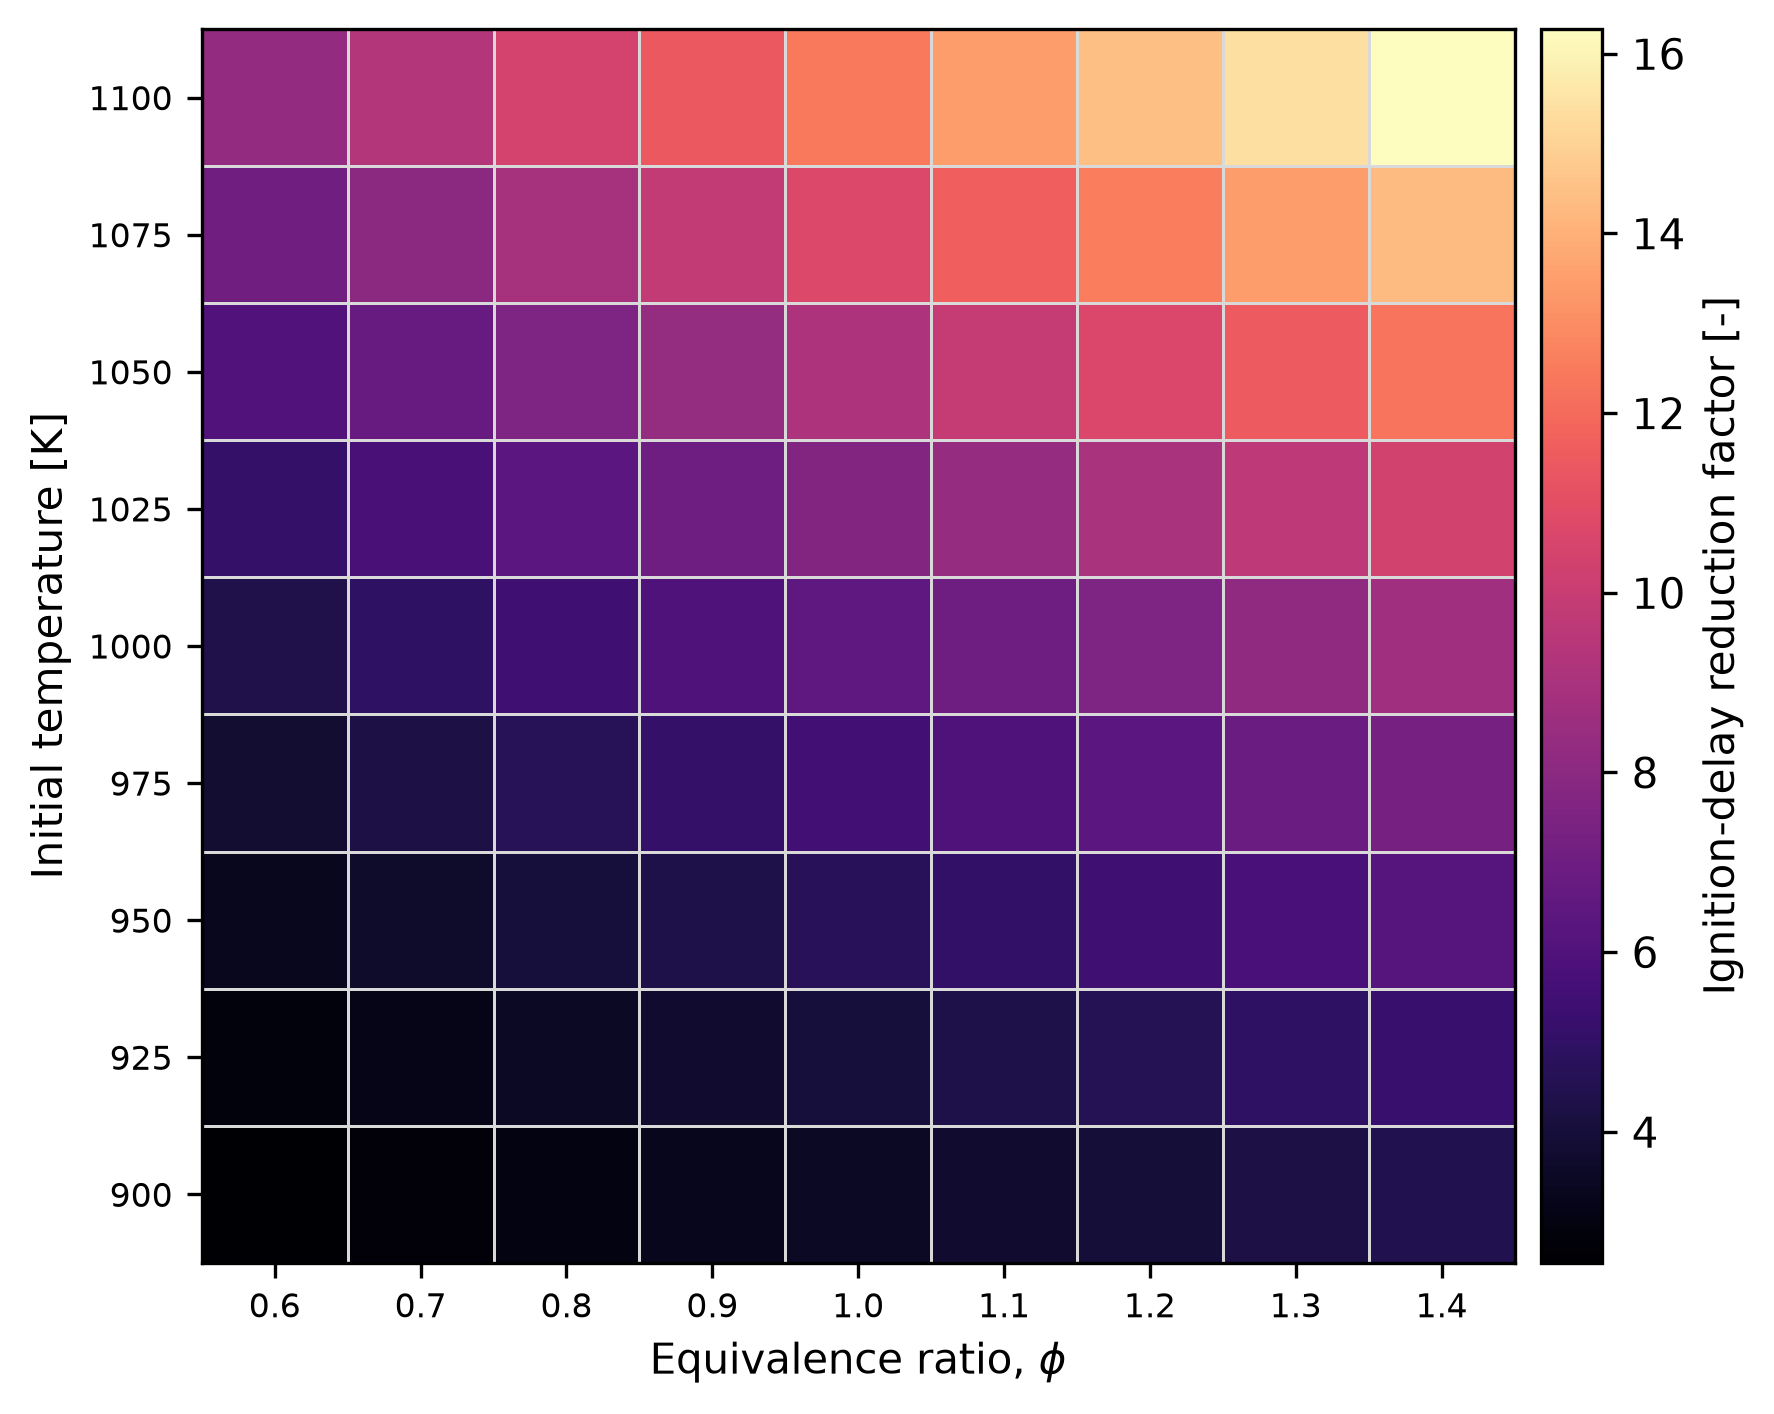
\includegraphics[width=0.88\textwidth]{ignition_delay_reduction_factor.png}
  \caption{Ignition-delay reduction factor
           $R_{\tau}=\frac{\tau_{\mathrm{ign},\,0\%\,\ce{H2}}}
           {\tau_{\mathrm{ign},\,40\%\,\ce{H2}}}$ for the same
           $T_0$--$\phi$ grid at $p=\SI{10}{\atmosphere}$. Values above one
           indicate a shorter calculated ignition delay for the
           \SI{40}{\mole\percent} hydrogen blend; the quantity is not an
           engine-efficiency or combustor-performance metric.}
  \label{fig:ign-reduction}
\end{figure}

\subsection{Constant-volume versus constant-pressure reactors}
The reactor-model comparison isolates the effect of the constant-volume versus
constant-pressure idealisation for the same mixtures and initial temperatures.
For all tested cases, the constant-pressure ignition delay is longer by
approximately 2.6\% to 8.8\%. The smallest difference is
2.60\% at $T_0=\SI{900}{\kelvin}$ and \SI{0}{\mole\percent} hydrogen
(\SI{586.74}{\milli\second} constant-volume versus
\SI{601.98}{\milli\second} constant-pressure), while the largest is
8.84\% at $T_0=\SI{1100}{\kelvin}$ and \SI{20}{\mole\percent} hydrogen
(\SI{2.05}{\milli\second} versus \SI{2.23}{\milli\second}). At
$T_0=\SI{1000}{\kelvin}$, the constant-pressure delays are
\SI{81.99}{\milli\second}, \SI{14.34}{\milli\second} and
\SI{12.64}{\milli\second} for 0, 20 and \SI{40}{\mole\percent} hydrogen,
compared with constant-volume values of \SI{79.74}{\milli\second},
\SI{13.41}{\milli\second} and \SI{11.86}{\milli\second}. The
constant-pressure reactor is therefore more representative of the adopted
combustor-oriented idealisation, but it is not a complete gas-turbine model.

\begin{figure}[tbp]
  \centering
  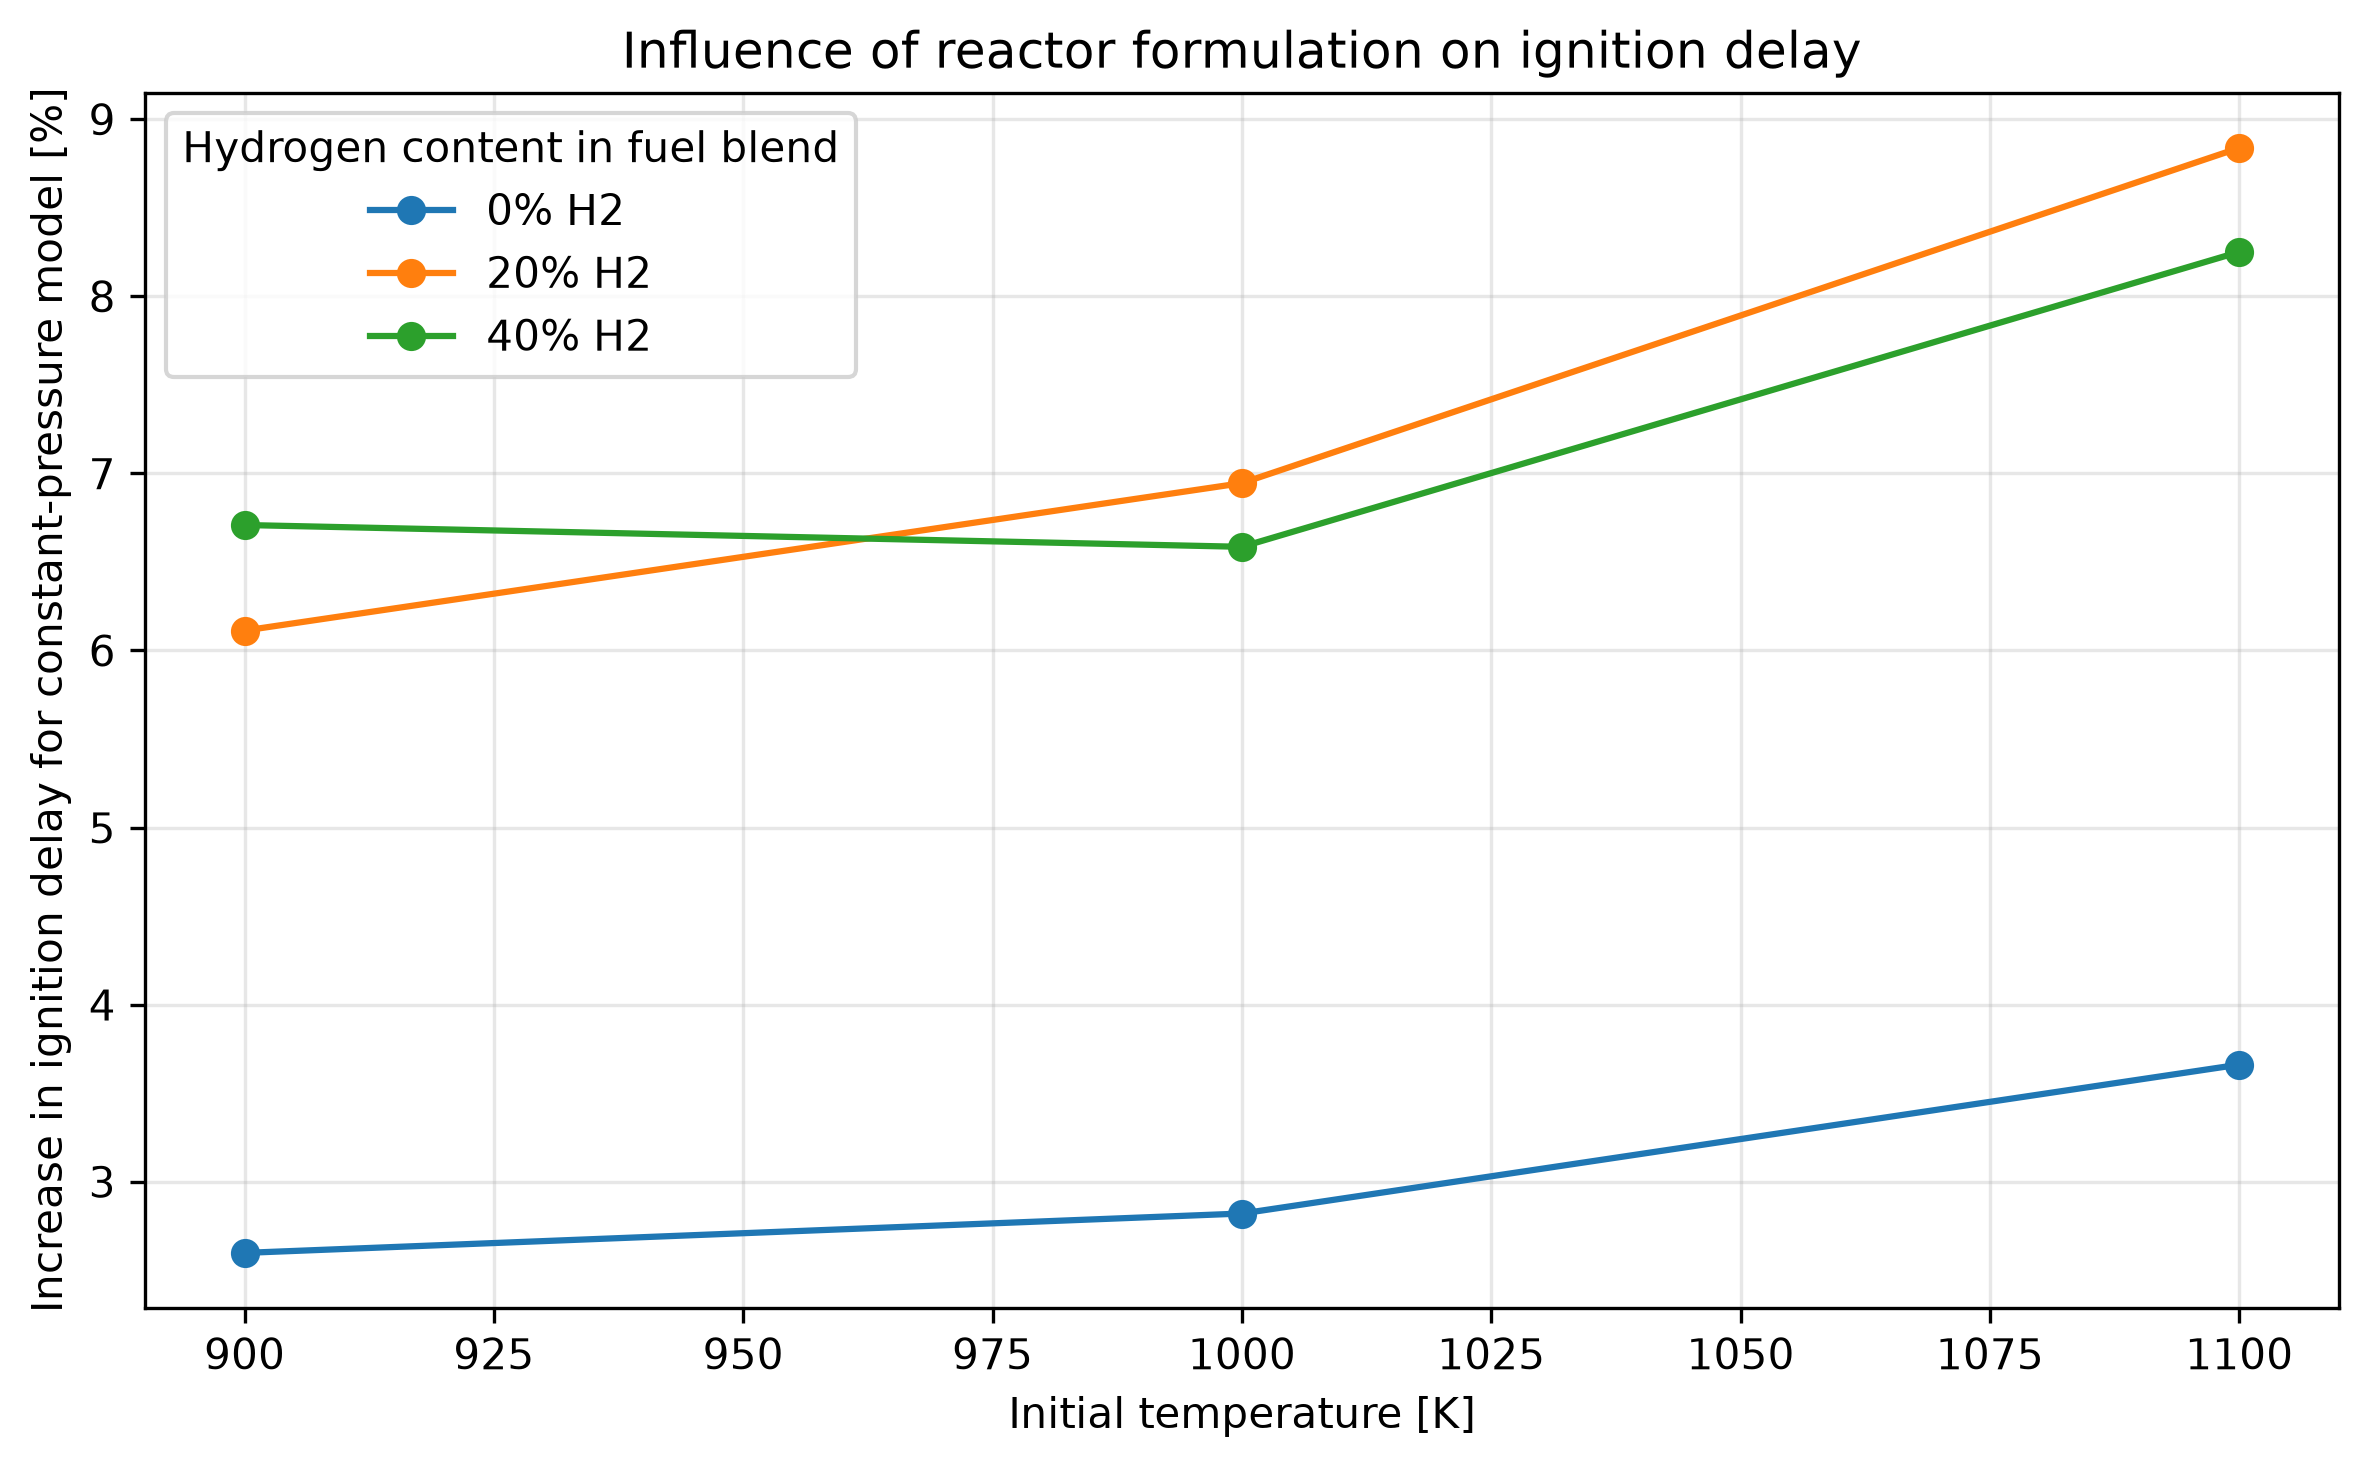
\includegraphics[width=0.82\textwidth]{reactor_model_comparison.png}
  \caption{Ignition delay at $\phi=1.0$ and $p=\SI{10}{\atmosphere}$:
           constant-volume versus constant-pressure reactor for
           $T_0=900$, 1000 and \SI{1100}{\kelvin}, and hydrogen fractions
           of 0, 20 and \SI{40}{\mole\percent}.}
  \label{fig:cvcp}
\end{figure}

\subsection{Laminar flame speed}
\label{sec:flamespeed}
The computed laminar flame speed of stoichiometric methane--air at reference
conditions is \SI{37.68}{\centi\meter\per\second}. This value is reported as
a result of the present \texttt{FreeFlame} model; no dedicated experimental
validation was performed. Hydrogen enrichment increases the calculated
stoichiometric flame speed to \SI{52.16}{\centi\meter\per\second} at
\SI{40}{\mole\percent} hydrogen in the fuel (Figure~\ref{fig:sl}).

\begin{figure}[tbp]
  \centering
  \begin{subfigure}{0.49\textwidth}
    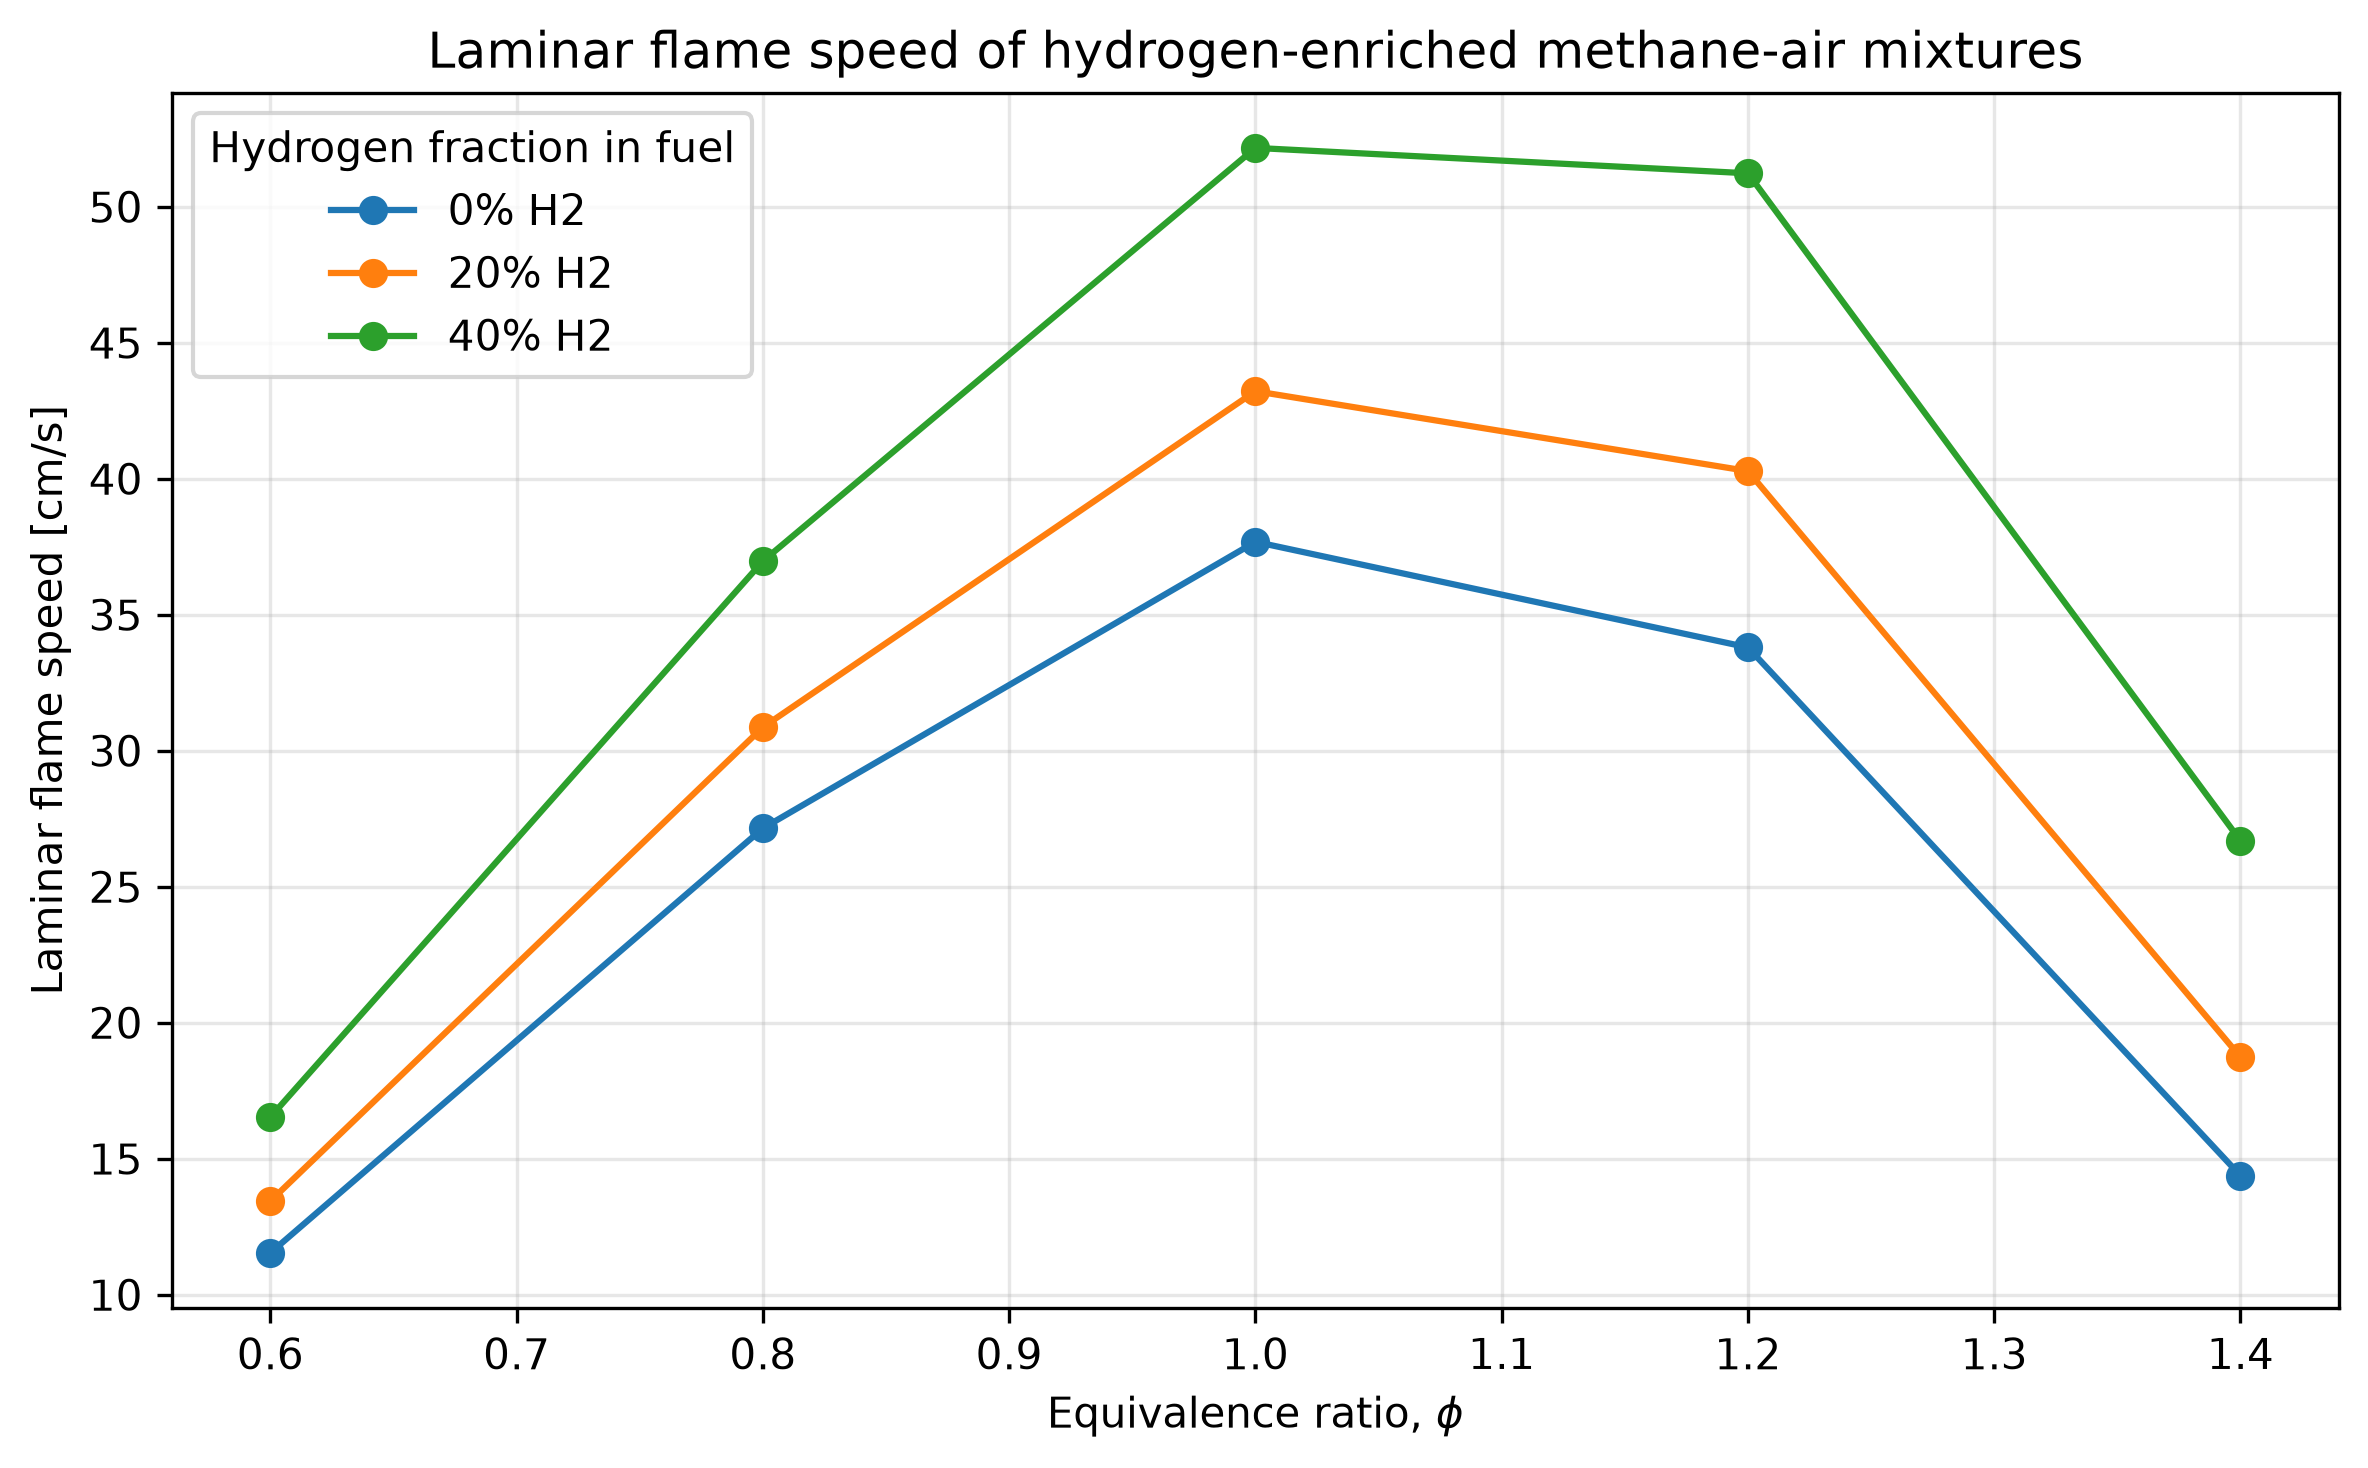
\includegraphics[width=\textwidth]{flame_speed_vs_equivalence_ratio.png}
    \caption{Versus equivalence ratio.}
  \end{subfigure}\hfill
  \begin{subfigure}{0.49\textwidth}
    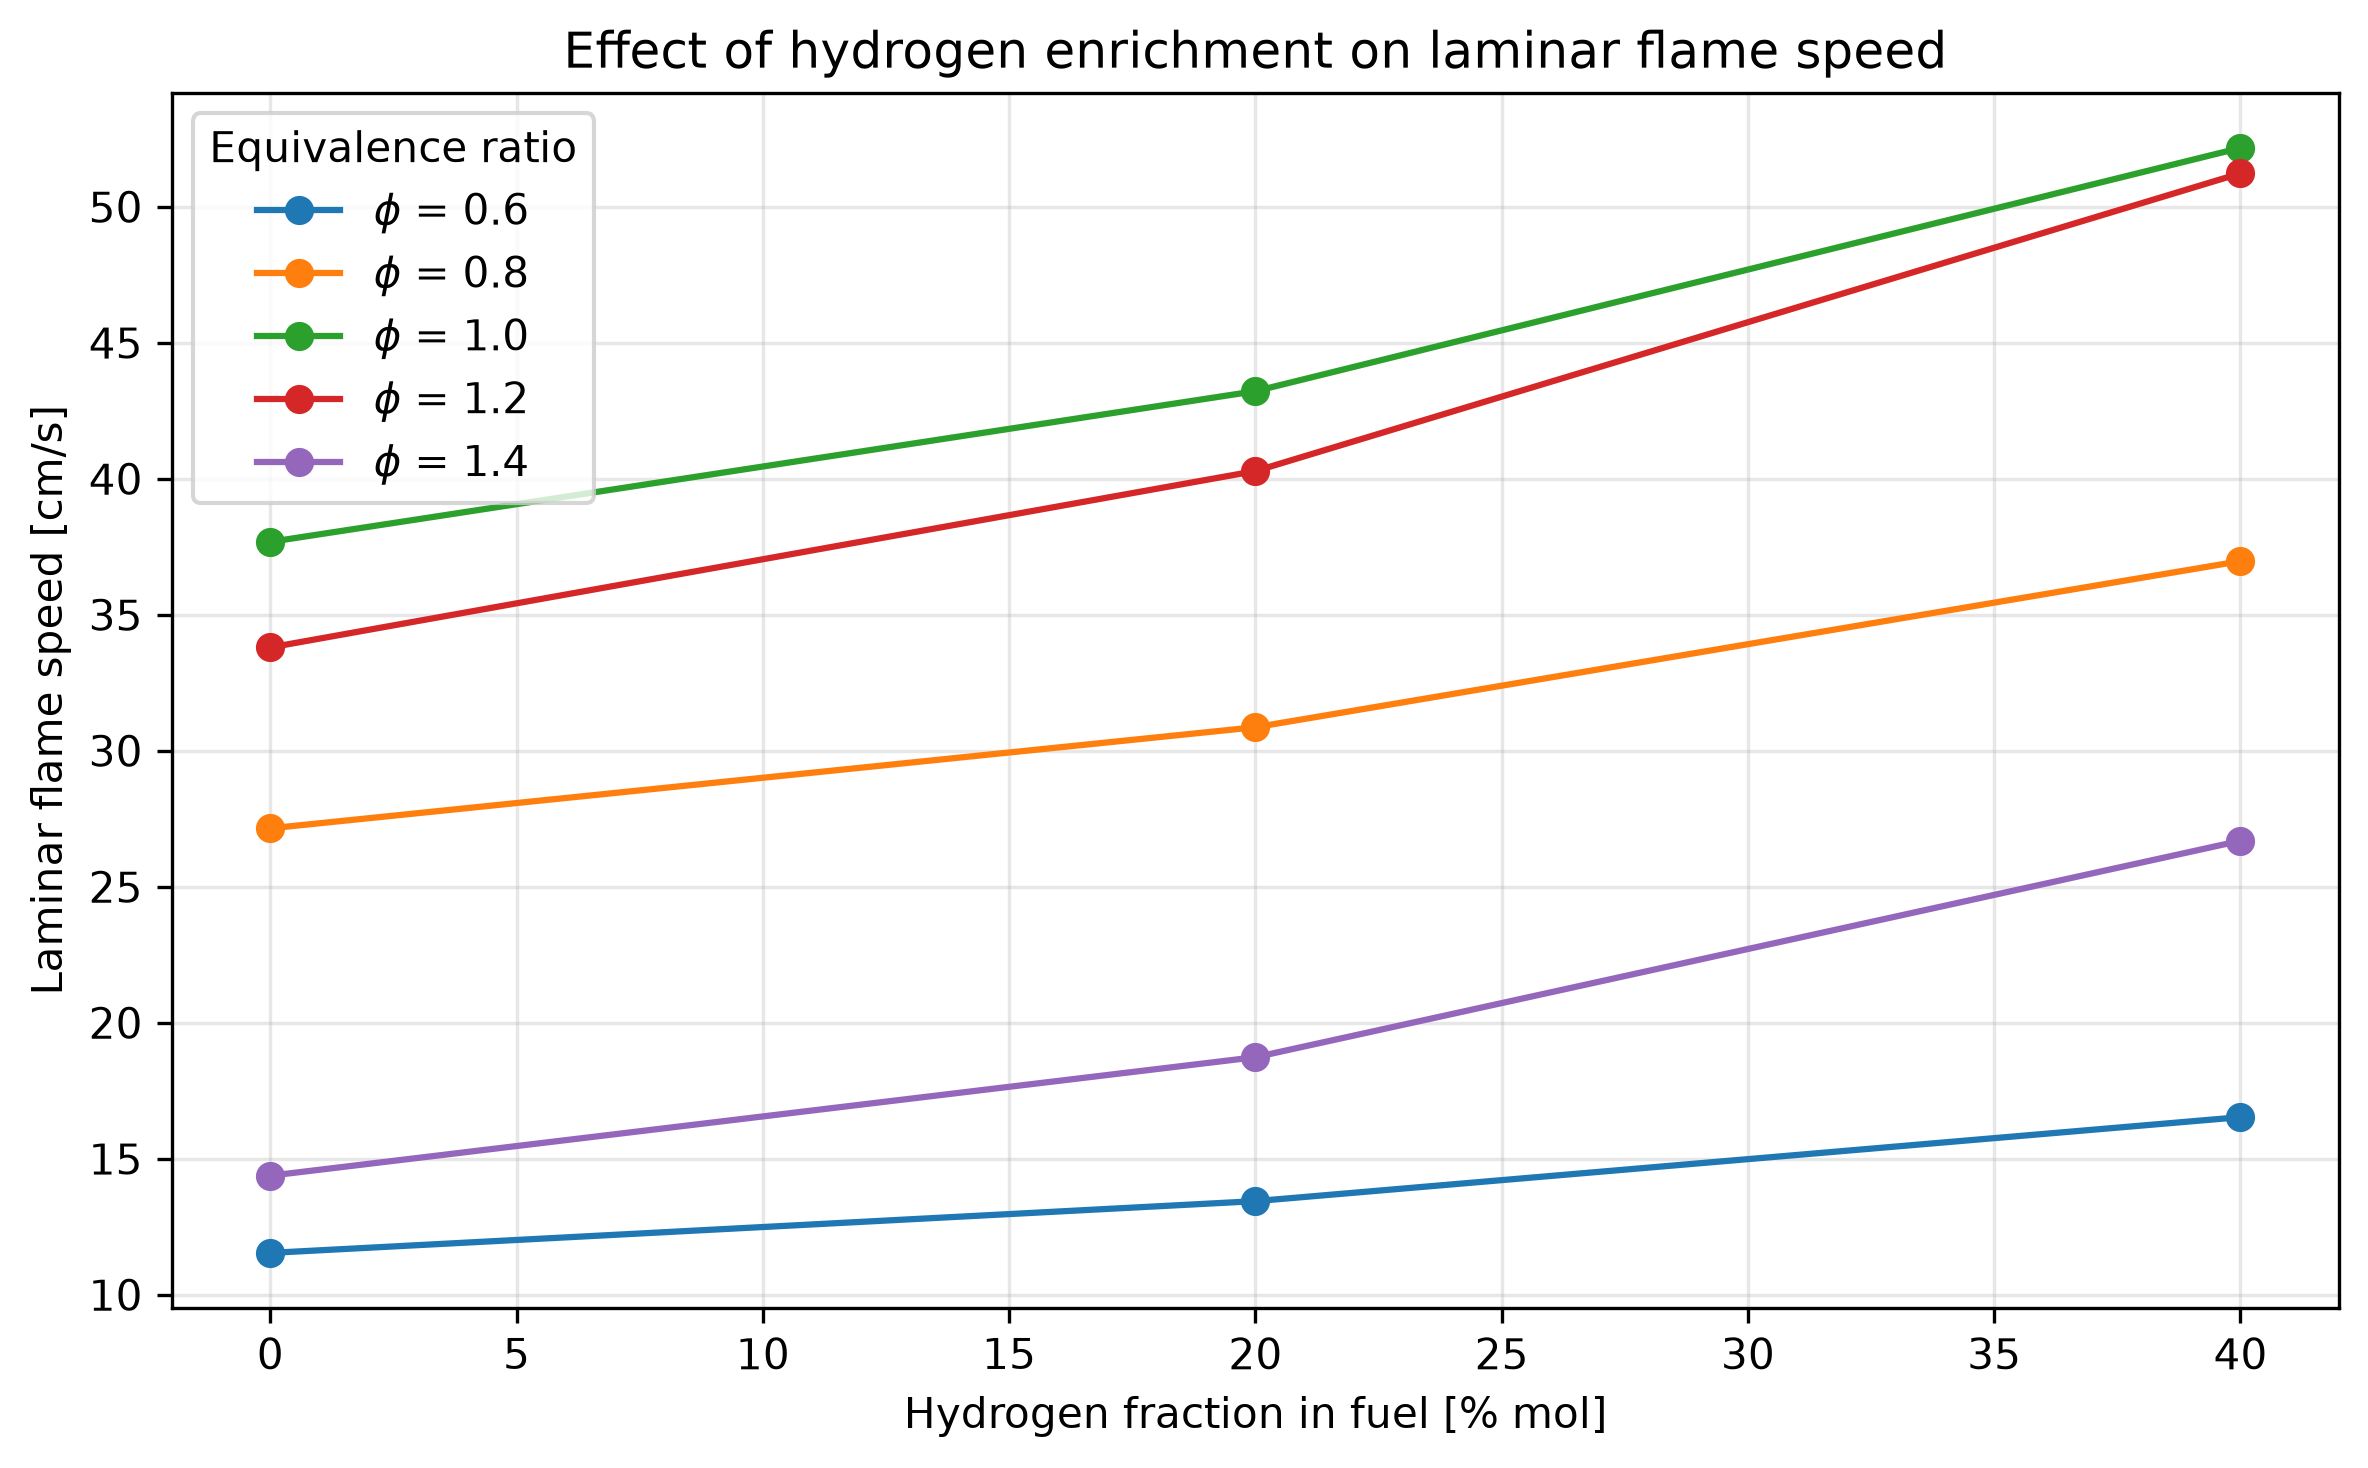
\includegraphics[width=\textwidth]{flame_speed_vs_h2_fraction.png}
    \caption{Versus hydrogen fraction.}
  \end{subfigure}
  \caption{Laminar flame speed of hydrogen-enriched methane--air flames.}
  \label{fig:sl}
\end{figure}

\subsection{Grid-refinement check}
The final flame-speed model uses multicomponent transport with Soret diffusion
enabled, so the diagnostic grid-refinement check was repeated with the same
transport settings rather than using earlier mixture-averaged calculations.
Two representative stoichiometric cases were compared: methane--air and the
\SI{40}{\mole\percent} hydrogen blend at \SI{300}{\kelvin} and
\SI{1}{\atmosphere}. The current setting uses ratio = 3.0, slope = 0.06 and
curve = 0.12; the tighter setting uses ratio = 2.5, slope = 0.03 and
curve = 0.06.

\begin{table}[htbp]
  \centering
  \caption{Diagnostic FreeFlame grid-refinement check using multicomponent
           transport and Soret diffusion.}
  \label{tab:grid-check}
  \begin{tabular}{llrrr}
    \toprule
    Case & Grid & $S_L$ [\si{\centi\meter\per\second}] &
    Points & Difference vs. tight [\%] \\
    \midrule
    \ce{CH4} & current & 37.68 & 197 & 0.75 \\
    \ce{CH4} & tight   & 37.40 & 359 & 0.00 \\
    40\% \ce{H2} & current & 52.16 & 202 & 0.19 \\
    40\% \ce{H2} & tight   & 52.07 & 382 & 0.00 \\
    \bottomrule
  \end{tabular}
\end{table}

For both representative cases, the current refinement settings differ from
the tighter grid by less than \SI{1}{\percent}, indicating limited sensitivity
of the reported flame speeds to further grid refinement.

\begin{figure}[tbp]
  \centering
  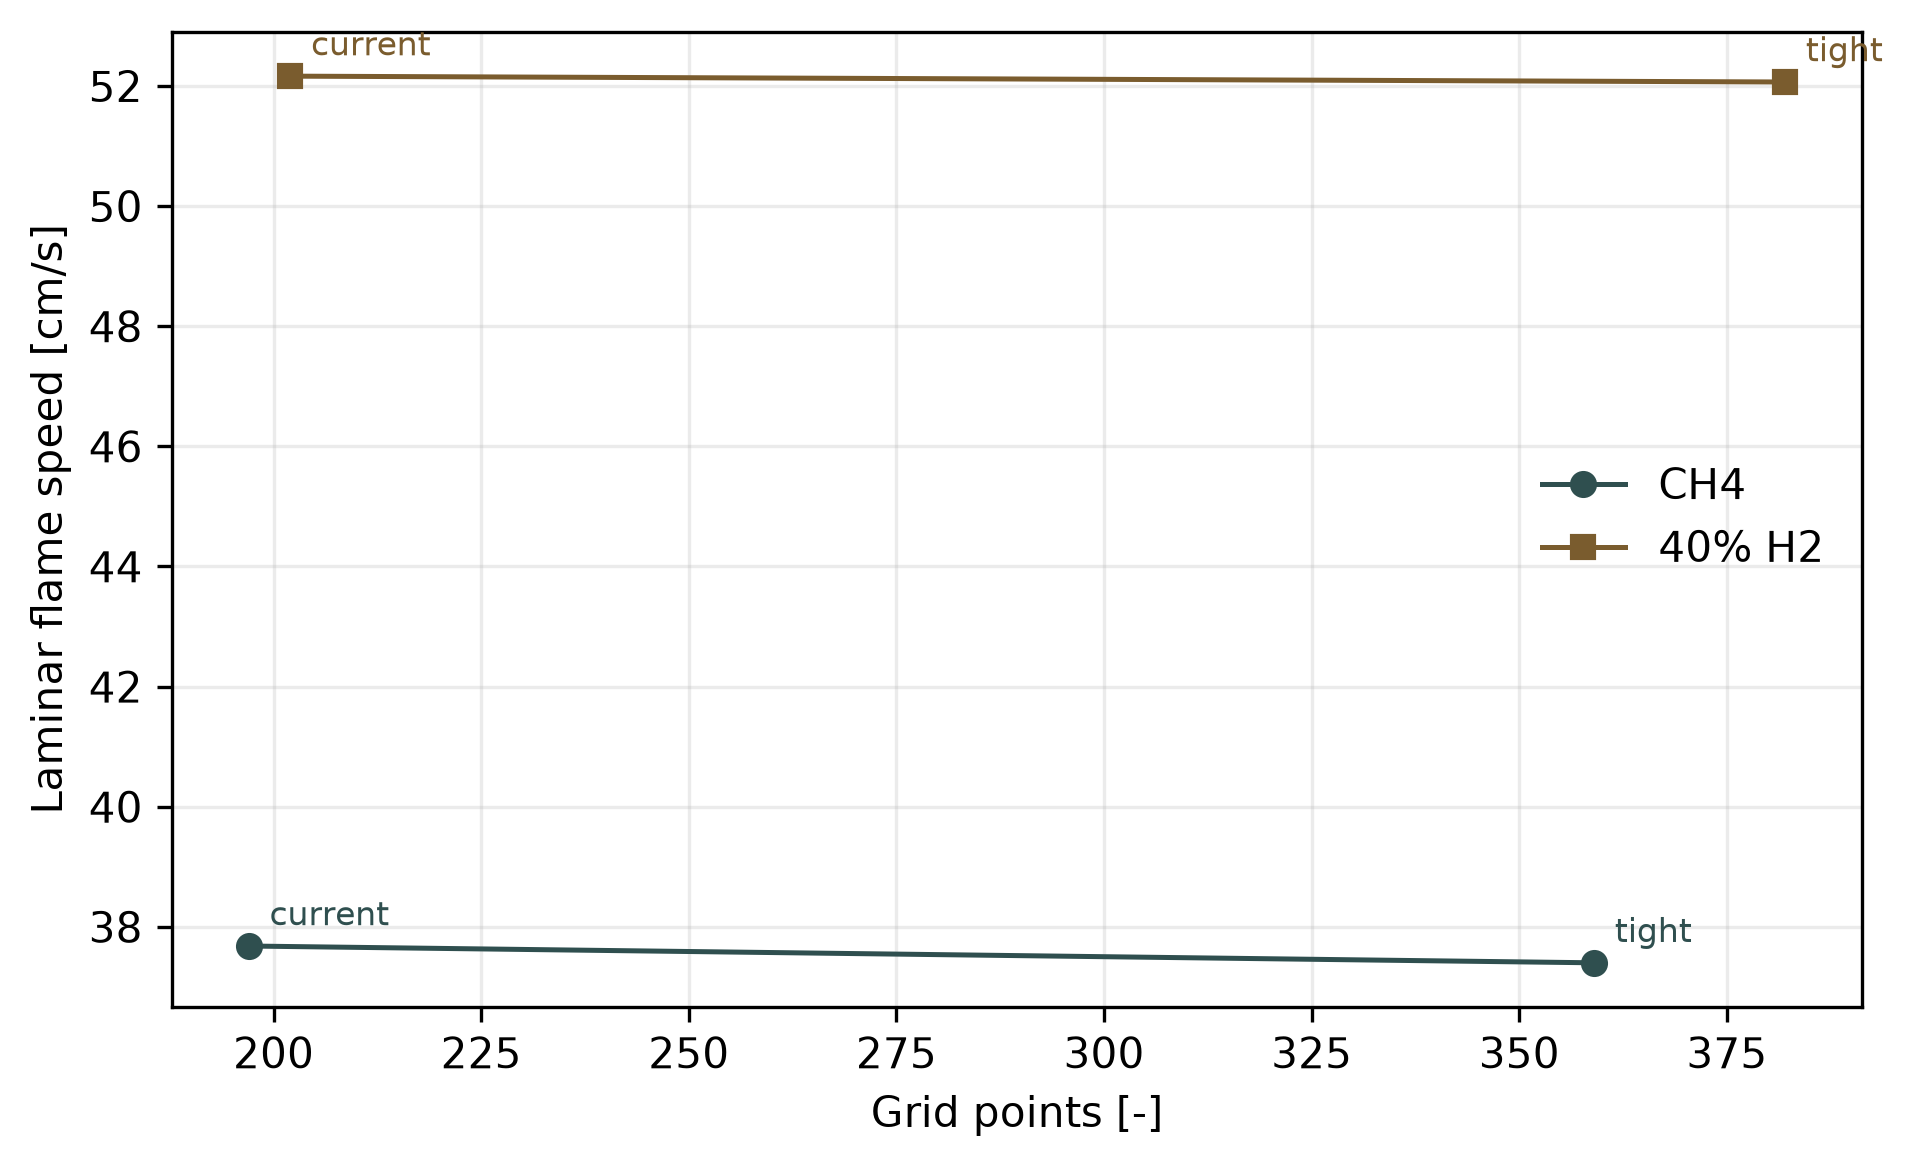
\includegraphics[width=0.76\textwidth]{flame_speed_grid_convergence.png}
  \caption{Diagnostic comparison of current and tight FreeFlame refinement
           settings. The check is a grid-refinement consistency check for two
           representative cases, not a validation against measurements.}
  \label{fig:grid-check}
\end{figure}

\subsection{Perfectly stirred reactor stability transition}
For each tested fuel blend and equivalence ratio, the PSR calculations provide
a stability-transition bracket between cold extinguished and hot stable
steady-state solutions on the tested residence-time grid. This ideal PSR
calculation does not represent actual engine behaviour, CFD, turbulence,
combustor geometry, recirculation or wall heat loss.

\begin{table}[htbp]
  \centering
  \caption{Discrete PSR stability-transition brackets on the tested
           residence-time grid.}
  \label{tab:psr-brackets}
  \begin{tabular}{cccc}
    \toprule
    $\phi$ & \ce{H2} in fuel [\si{\mole\percent}] &
    Extinguished $\tau$ [\si{\milli\second}] &
    Stable $\tau$ [\si{\milli\second}] \\
    \midrule
    0.7 & 0  & 0.005 & 0.010 \\
    0.7 & 20 & 0.002 & 0.005 \\
    0.7 & 40 & 0.002 & 0.005 \\
    1.0 & 0  & 0.002 & 0.005 \\
    1.0 & 20 & 0.002 & 0.005 \\
    1.0 & 40 & 0.002 & 0.005 \\
    \bottomrule
  \end{tabular}
\end{table}

These values are discrete brackets from the configured residence-time grid,
not resolved transition times. Hydrogen enrichment moves the
observed bracket for the lean $\phi=0.7$ case from 0.005--\SI{0.010}{\milli\second}
for methane--air to 0.002--\SI{0.005}{\milli\second} for the enriched cases;
at $\phi=1.0$, all three tested fuel blends share the same
0.002--\SI{0.005}{\milli\second} bracket.

\begin{figure}[tbp]
  \centering
  \begin{subfigure}{0.78\textwidth}
    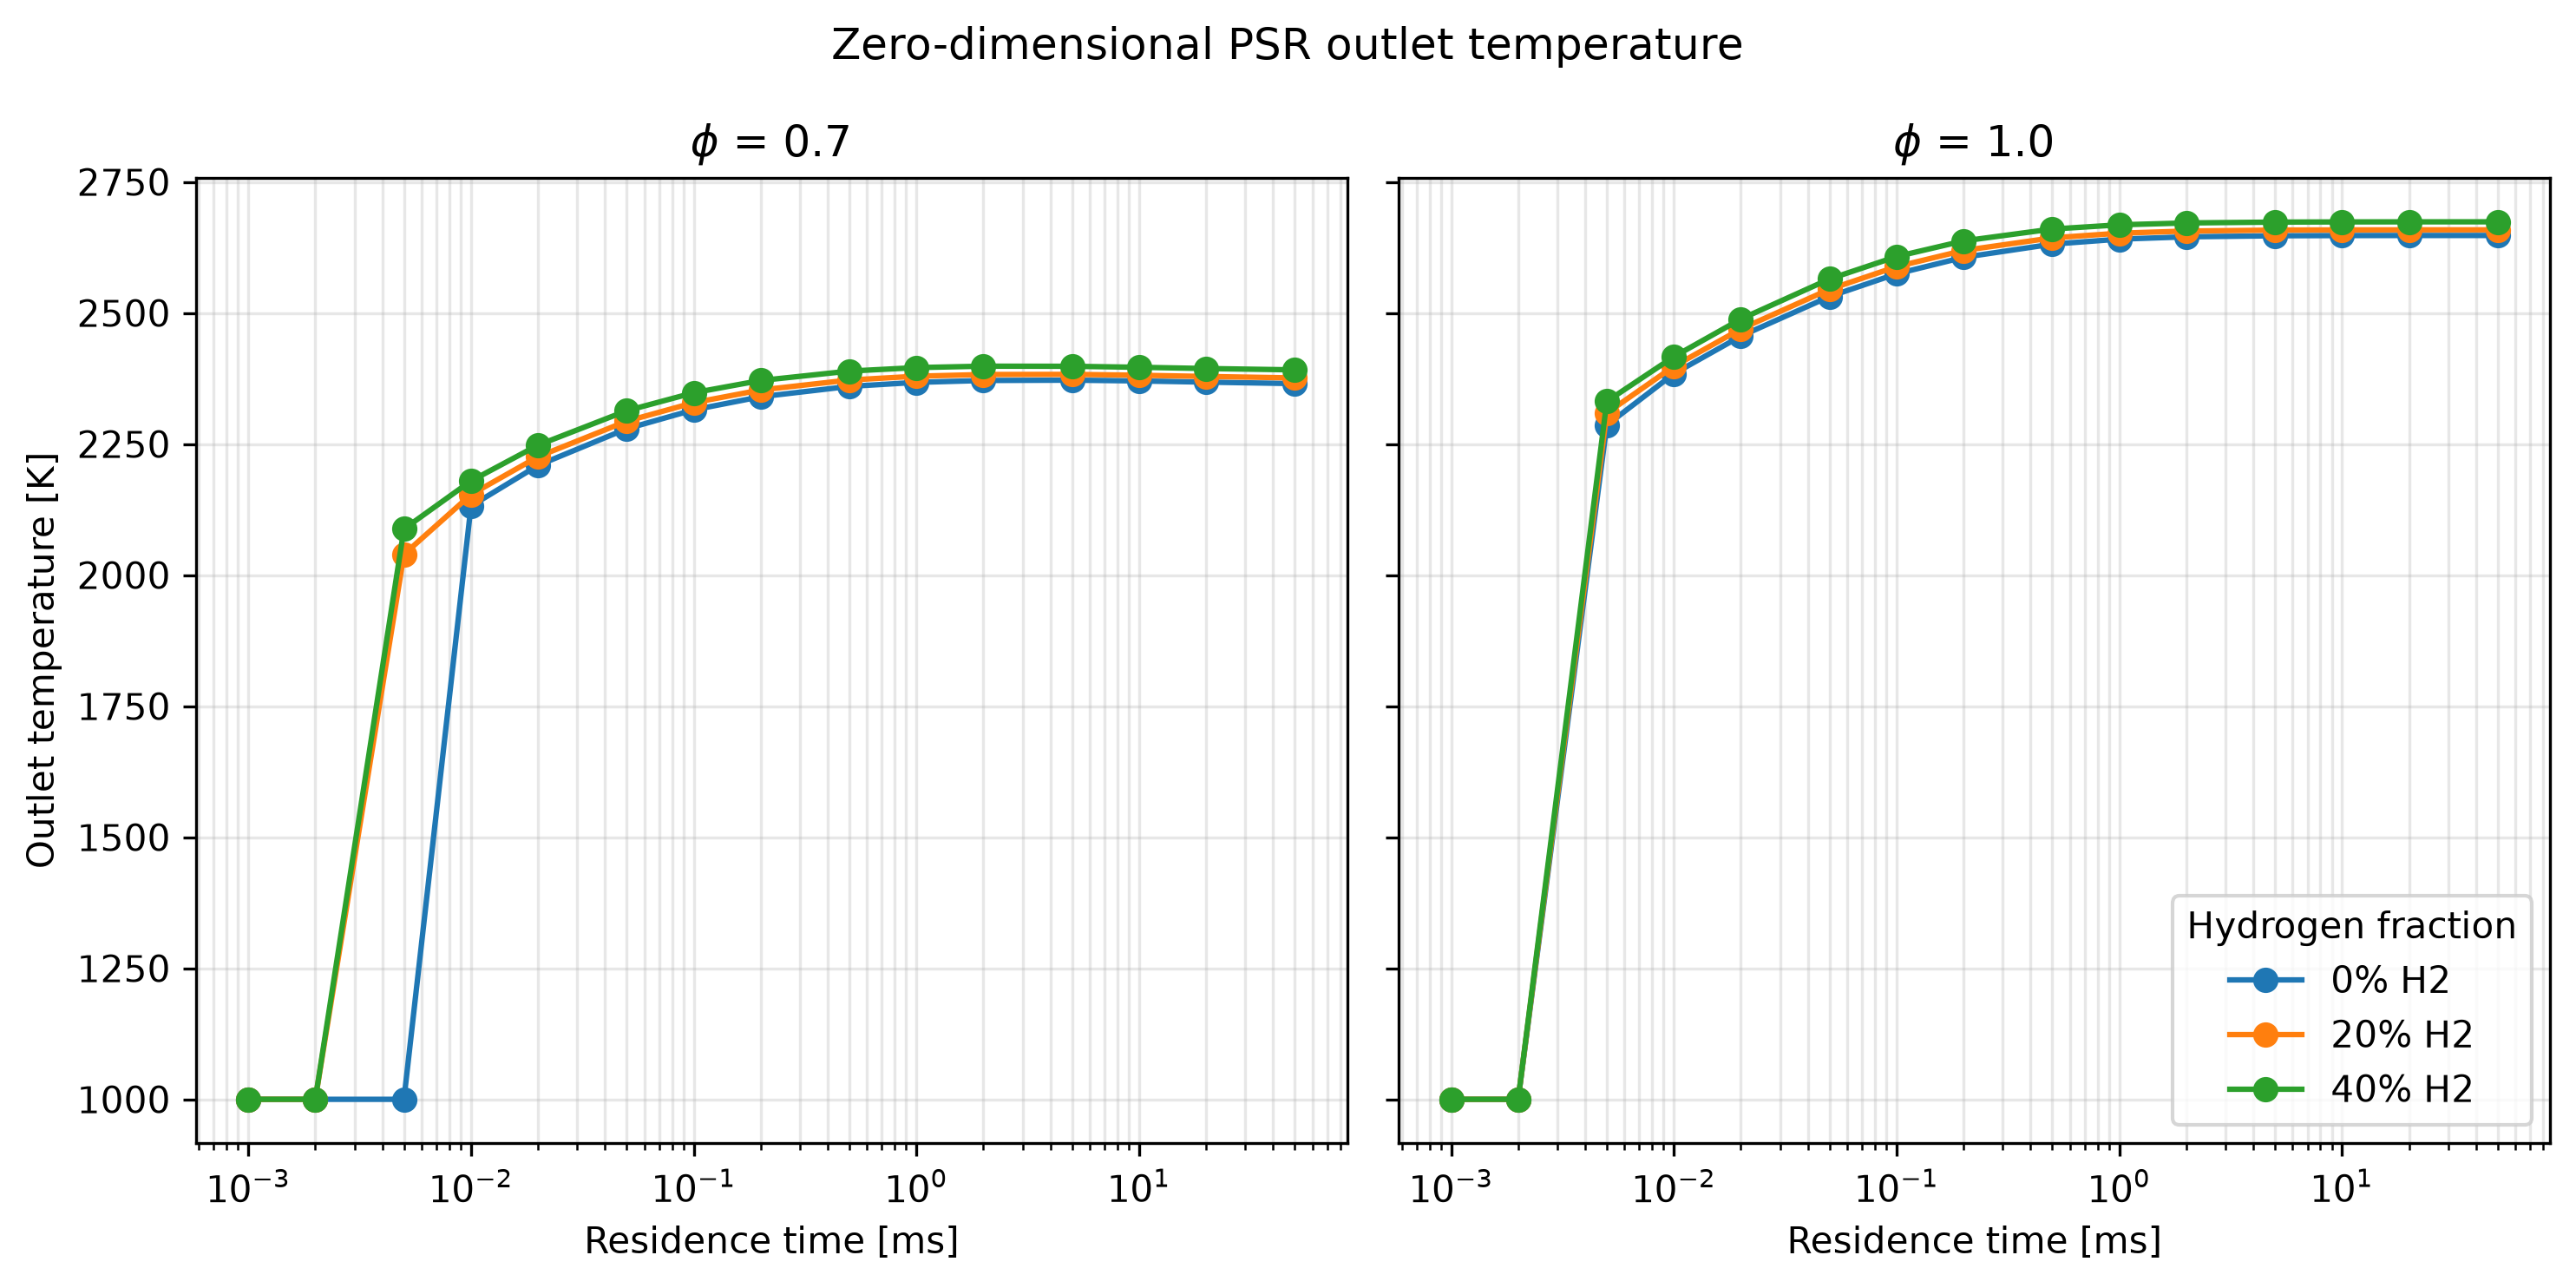
\includegraphics[width=\textwidth]{combustor_temperature_vs_residence_time.png}
    \caption{Outlet temperature.}
  \end{subfigure}

  \begin{subfigure}{0.78\textwidth}
    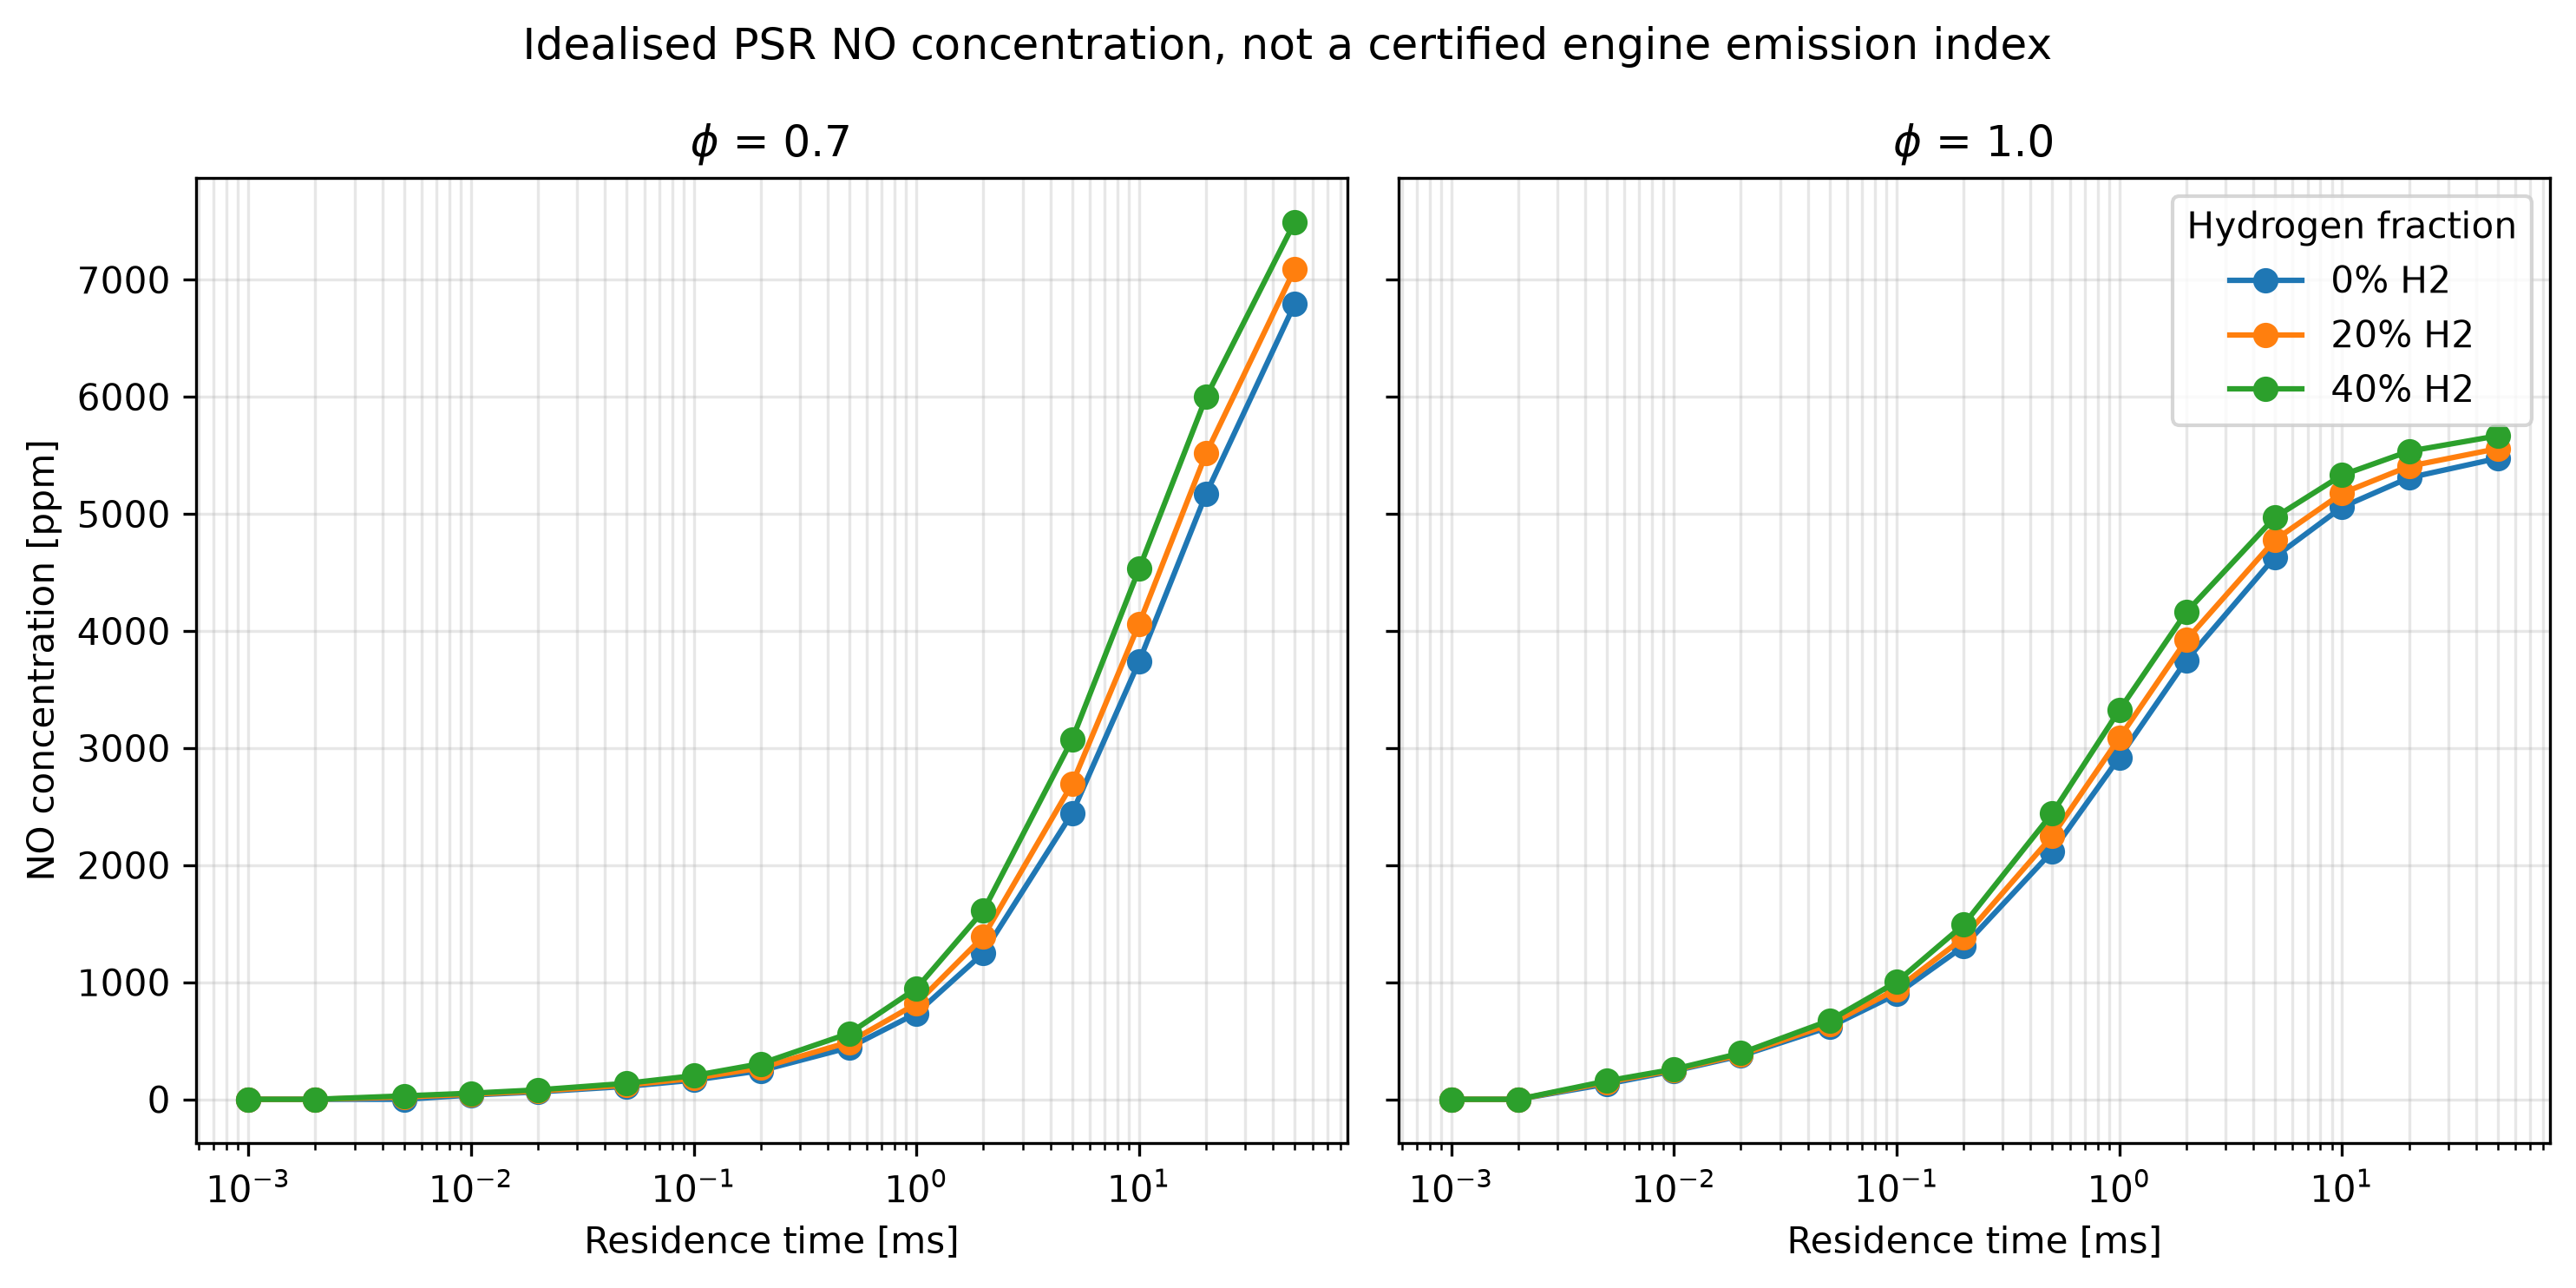
\includegraphics[width=\textwidth]{combustor_no_vs_residence_time.png}
    \caption{\ce{NO} mole fraction.}
  \end{subfigure}
  \caption{PSR behaviour versus residence time; the drop at short residence
           time marks a stability-transition bracket on the tested grid.
           Inlet conditions are $T_\mathrm{in}=\SI{1000}{\kelvin}$,
           $p=\SI{10}{\atmosphere}$, with $\phi=0.7$ and 1.0.}
  \label{fig:psr}
\end{figure}

\begin{figure}[tbp]
  \centering
  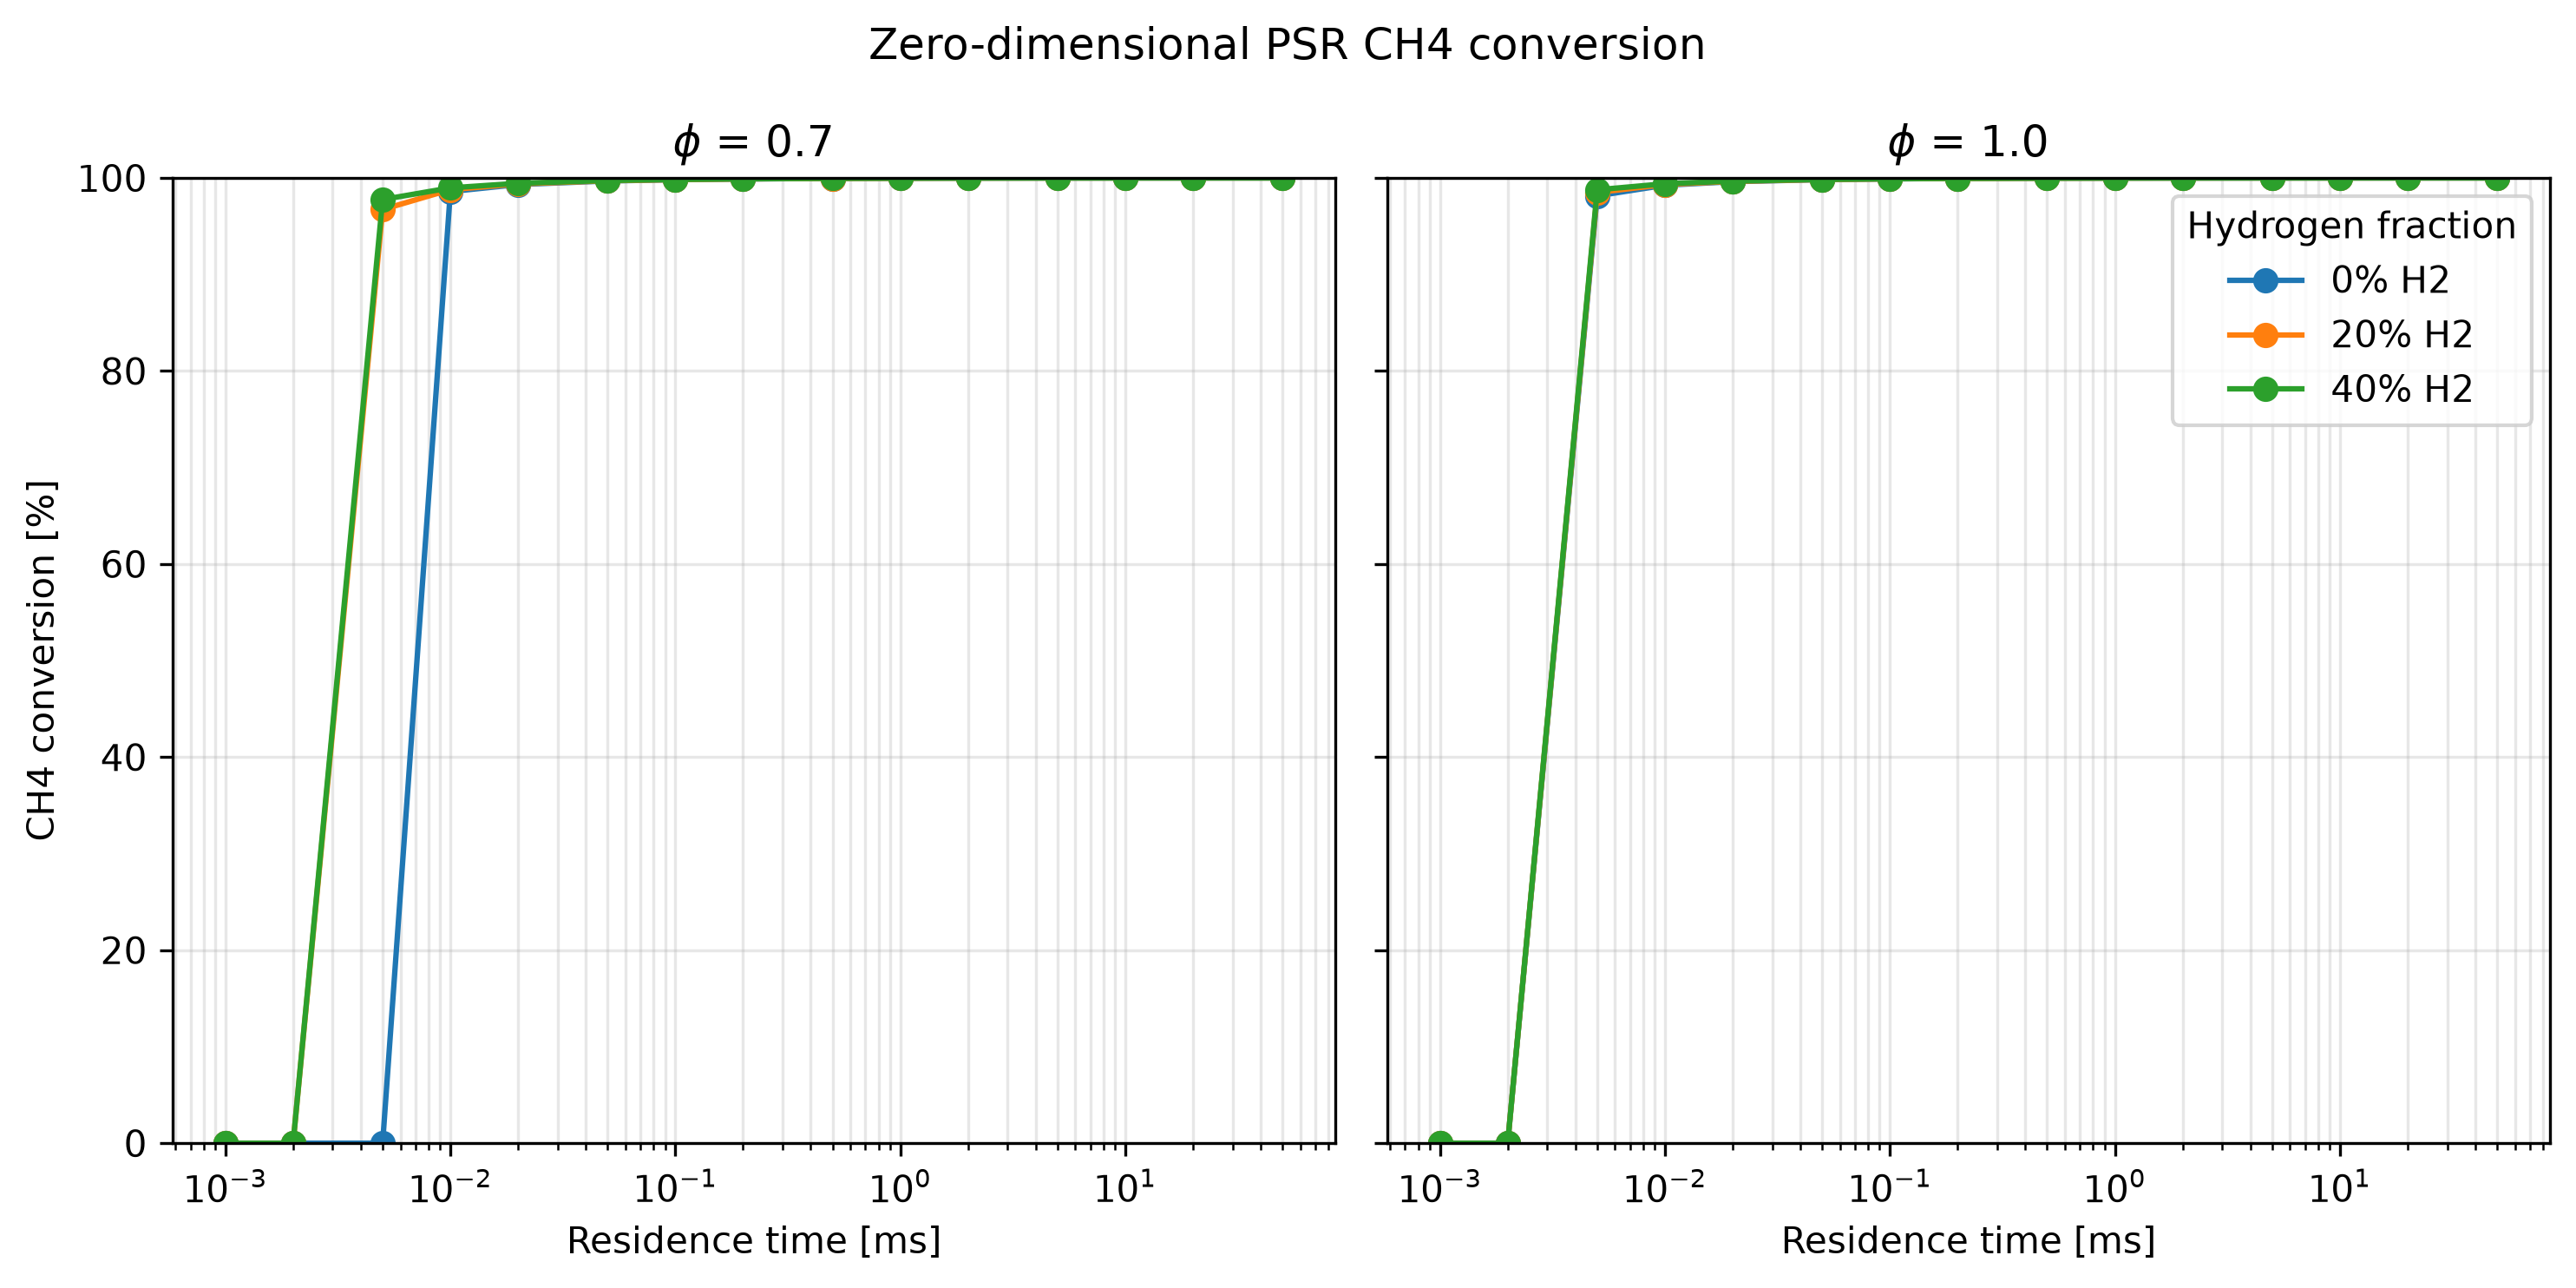
\includegraphics[width=0.82\textwidth]{combustor_ch4_conversion_vs_residence_time.png}
  \caption{Ideal PSR \ce{CH4} conversion versus residence time at
           $T_\mathrm{in}=\SI{1000}{\kelvin}$,
           $p=\SI{10}{\atmosphere}$, $\phi=0.7$ and 1.0. Conversion is shown
           only as a finite-rate stirred-reactor trend; it does not include
           mixing, geometry, wall heat loss or turbine-combustor residence
           time distributions.}
  \label{fig:psr-conversion}
\end{figure}

\FloatBarrier

% ===========================================================================
\section{Model limitations and conclusions}

\subsection{Model limitations}
\label{sec:limitations}
GRI-Mech~3.0 was optimised and validated for natural-gas (methane-dominated)
combustion \citep{grimech30}. For the hydrogen fractions considered here
($x_{\ce{H2}} \le 0.4$), the mixture remains methane-dominated, so its use is
defensible; however, for higher hydrogen content a dedicated hydrogen
mechanism, such as that of \citet{burke2012} or \citet{oconaire2004}, would be
more appropriate. The flame-speed calculations use multicomponent transport
with Soret diffusion, but they still represent one-dimensional, freely
propagating, adiabatic premixed flames. The PSR is zero-dimensional, adiabatic
and perfectly stirred, with no representation of actual engine operation, CFD,
turbulence, geometry, recirculation or wall heat loss. The equilibrium
calculations also assume infinite-time chemical equilibrium and therefore
cannot represent finite-rate effects in the nozzle/exhaust.

\subsection{Conclusions}
\begin{enumerate}
  \item At $\phi=1.0$, \SI{300}{\kelvin} and \SI{1}{\atmosphere}, increasing
  the fuel hydrogen fraction from \SI{0}{\percent} to \SI{40}{\percent}
  increased the calculated laminar flame speed from
  \SI{37.68}{\centi\meter\per\second} to
  \SI{52.16}{\centi\meter\per\second}.

  \item At $T_0=\SI{1000}{\kelvin}$, $p=\SI{10}{\atmosphere}$ and $\phi=1.0$,
  the constant-pressure ignition delay decreased from
  \SI{81.99}{\milli\second} for methane--air to
  \SI{12.64}{\milli\second} for the \SI{40}{\percent} hydrogen blend.

  \item For the tested PSR grid, cold extinguished and hot stable
  steady-state solutions were separated by a stability-transition bracket in
  residence time, rather than by a resolved exact transition point.

  \item The present results are limited to detailed-chemistry idealisations:
  equilibrium reactors, homogeneous ignition calculations, one-dimensional
  freely propagating flames and a zero-dimensional adiabatic PSR.

  \item In a simplified combustor-screening sense, hydrogen enrichment in the
  tested \ce{CH4}/\ce{H2} blends tends to accelerate ignition and increase
  flame speed, so it should be evaluated together with stability margins,
  thermal loading and emissions constraints before any hardware-level
  interpretation.
\end{enumerate}

\clearpage

% ===========================================================================
\phantomsection
\addcontentsline{toc}{section}{Bibliography}
\bibliographystyle{unsrtnat}
\bibliography{references}

\end{document}
